\documentclass{tran-l}
\usepackage{amssymb}
\usepackage{mathrsfs}
\usepackage{xcolor}
\usepackage{graphicx}
\usepackage{subcaption}

\newtheorem{theorem}{Theorem}
\newtheorem{lemma}[theorem]{Lemma}

\theoremstyle{definition}
\newtheorem{definition}[theorem]{Definition}
\newtheorem{example}[theorem]{Example}
\newtheorem{xca}[theorem]{Exercise}

\theoremstyle{remark}
\newtheorem{rem}{Remark}
\newtheorem{requ}{Research Question}

\numberwithin{equation}{section}

%    Absolute value notation
\newcommand{\abs}[1]{\lvert#1\rvert}

%    Blank box placeholder for figures (to avoid requiring any
%    particular graphics capabilities for printing this document).
\newcommand{\blankbox}[2]{%
  \parbox{\columnwidth}{\centering
%    Set fboxsep to 0 so that the actual size of the box will match the
%    given measurements more closely.
    \setlength{\fboxsep}{0pt}%
    \fbox{\raisebox{0pt}[#2]{\hspace{#1}}}%
  }%
}

\newcommand{\mR}{\mathbb{R}}

\title{Meta-Learning with Kernel Ridge}

\begin{document}

\maketitle

\rem This may be an oversimplification but here it goes...  A conventional learning problem where the aim is to estimate a ground truth from several observations. In a meta-learning problem, we have a distribution of learning tasks (Let's not specify anything regarding the distribution yet). In this given case we can observe a set of conventional learning problems with their specific observations. We are still interested in a single learning task, but we assume that we can leverage some information coming from other learning tasks originating from the same learning problem distribution. 

Well, the story of meta-learning starts with LSTMs, etc. But these days they turned into smart initialization finding for the distribution of tasks at hand. For deep learning applications. The "Learning Around a Common Mean" paper creates a convex meta-learning model where all the parameters of the model are adjusted for the task distribution. In the meta-learning settings achieving this convex problem is not abundant (Especially in a nonlinear problem setting where you cannot use linear models effectively.).


\rem In our investigation of the MAML we have observed that this Ridge-based meta-learning method can achieve more stable results compared to SGD-based meta-learning methods. However, we are only able to observe this in the linear setting as there is no non-linear version present. Then, I asked the question with a similar penalization technique used in the "Learning Around the Common Mean" paper;
 
\requ Can a convex kernelized meta-learning method be constructed that can learn some of its parameters from task distribution and has a comparable or better performance and is more interpretable compared to conventional deep learning based meta-learning models in a few-shot learning setting (where there is a limited number of data available from a task of interest coming from the same task distribution)?

\requ If we can create a model like that can we give statistical guarantees under specific assumptions that the expected risk of this model will be better than its conventional counterpart on a given learning task?

Well, I acknowledge that it might be too ambitious for a research question, and in the end what I am doing ended up not being a convex problem but still I believe there are still some interesting research questions moving forward. (Apparently it is not that ambitious for some of you. Then, I wonder why I do not see any method like this? And although it is not ambitious then I still find it hard to come up with a model that is capable of solving this type of problem.) So, please bear with me maybe I can convince you at least to a certain extent that meta-learning can be useful in certain extrapolation problems. 

\section{Basic Setup}

A task $T_a$ is a $d$-dimensional regression problem in which the input-output relation is given by

\begin{equation}\label{eq:data}
y = f_a(\mathbf{x}) + \varepsilon,
\end{equation}
where $y\in\mR$, $\mathbf{x} \in \mR^d$, and $\varepsilon$ is taken to be standard normal.  The task space is defined by a distribution $p_f$ over functions. 

\rem I am not considering any specific distribution over functions for now. However, we can consider a Gaussian Process $f(\mathbf{x}) \sim GP(m(\mathbf{x}), cov(\mathbf{x},\mathbf{x}^\prime))$ as a distribution over functions for instance.

Let us assume that the input distribution is denoted as $p_{\mathbf{x}}$ and for every task, we have the same input distribution. Moreover,  we have observed $N_a$ samples from the corresponding regression problem which are collected in
\begin{equation}
Z_a:=\left((\mathbf{x}_i,y_i)\right)_{i=1}^{N_a}.
\end{equation}

For the time being, the loss we consider is the standard least squares loss, as for now my interest lies with the regression problems ($\mathcal{L}_a=\sum_i^{N_a}(\hat{f}(\mathbf{x}_i)-y_i)^2$).

\rem Now, with Marco's reading suggestions I ended up finding the two approaches to incorporate the information gained from tasks $p_f$ (noting that I am still not specifying $p_f$ on purpose) to improve the prediction of $T_a$. The first method uses the Semi-parametric Representer Theorem and the second method is Biased Regularization. The reason we are only considering these two approaches is to see if we can extend the "Learning Around a Common Mean" paper to a nonlinear setting while still preserving the convex problem setting. In the end, we might need to of course select other methods to compare our method, but for now, there are two options that I suspect have the stability and the performance of their linear counterpart which can perform better than most used meta-learning problems in the nonlinear setting. I have not encountered any kernel-based meta-learning model, especially with the construction that I have in mind. I am wondering why other people have not pursued this path.

Let us first start with the method that uses Semi-parametric Representer Theorem. 

\section{Method}

\rem For the sake of brevity let's forget about the so-called task space of the meta-learning problem and focus on the single learning problem $T_a$. Where we are trying to learn $f_a(\mathbf{x})$. Then, from now on I will abuse the notation and will use $\hat{f}_a(\mathbf{x})\triangleq f $ for our estimator. \\

Thanks to Nonparametric Representer Theorem for $g$ to be a strictly increasing function and $\mathcal{L}$ being a monotonic loss function, then 
\begin{equation}
  \hat{f} = \min_{f\in\mathcal{H}}\quad \sum_i^{N_a}(f(\mathbf{x}_i)-y_i)^2 + g(||f||_\mathcal{H})
\end{equation} 
has the solution of the form, $f(\cdot)=\sum^{N_a}_i\alpha_i k(\cdot,\mathbf{x}_i)$ \footnote{Here $\mathcal{H}$ represents the Reproducing Kernel Hilbert Space}. This is the most fundamental step to kernalize the Linear Ridge Regression method.
%(I know you will say we called our estimator $f$ what happened now, but I am assuming that f estimator is only related to observed dataset $Z_a\triangleq Z$.). 
In the Semi-parametric Representer Theorem  $\tilde{f}= f + h$ where $h\in span\{\psi_p\}$ and $\{\psi_p\}_{p=1}^M$ are real-valued functions and $\mathcal{L}=\sum_i^N(\tilde{f}(\mathbf{x}_i)-y_i)^2$. Then the solution to 
\begin{equation}
\hat{\tilde{f}} = \min_{\tilde{f}\in\mathcal{H}}\quad\sum_i^{N_a}(\tilde{f}(\mathbf{x}_i)-y_i)^2 + g(||f||_\mathcal{H})
\end{equation}  
has the form $\tilde{f}(\cdot)=\sum^N_i\alpha_i k(\cdot,\mathbf{x}_i)+\sum_j^M\beta_j\psi_j(\cdot).$

In other words, on top of our observed dataset, $Z_a\triangleq Z$ we are given real-valued functions $\{\psi_p\}_{p=1}^M$ and our final estimator will use data points and extra information coming from multiple functions for the estimator $\tilde{f}$. 

\rem  You might wonder; "Why are we doing this?",  "What does it mean in the sense of meta-learning?". Well, as I have stated earlier we have access to the observations from the task space. Because of this, we might be able to put meta-information via those functions $\{\psi_p\}_{p=1}^M$ for now I am not specifying anything again. However, one might imagine that we might use trained models, simple interpolation (If there is enough data available of course), or exact functions if we have access to those. Then with this procedure, we will be technically weighing them with the observed data to come up with our estimator for a specific task at hand.

Well after some tiny bit of taking derivatives and equating to zero for $g(||f||_\mathcal{H}):=\lambda||f||^2$, the optimal solutions are given by:

\text{Nonparametric Representer Theorem}:
\begin{equation}
 \hat{\boldsymbol{\alpha}}=(\mathbf{K}+\lambda \mathbf{I})^{-1}\mathbf{y}
\end{equation}

and \\

\text{Semiparameteric Representer Theorem}: 
\begin{align}
  \hat{\boldsymbol{\alpha}}&=(\mathbf{K}\mathbf{K}+\lambda\mathbf{K}-\mathbf{K}\boldsymbol{\psi}(\boldsymbol{\psi}^\text{T}\boldsymbol{\psi})^{-1}\boldsymbol{\psi}^\text{T}\mathbf{K})^{-1}(\mathbf{K}-\mathbf{K}\boldsymbol{\psi}(\boldsymbol{\psi}^\text{T}\boldsymbol{\psi})^{-1}\boldsymbol{\psi})\mathbf{y} \\ 
  \hat{\boldsymbol{\beta}}&=(\boldsymbol{\psi}^\text{T}\boldsymbol{\psi})^{-1}(\boldsymbol{\psi}^\text{T}\mathbf{y}-\boldsymbol{\psi}^\text{T}\mathbf{K}\hat{\boldsymbol{\alpha}})
\label{eq:optimum}
\end{align}

\rem Again, abusing the notations to the fullest extent but the bold letters represent the collections of the values of the non-bold versions in row vectors as follows;
$\boldsymbol{\alpha}\in\mR^{N_a\times 1}$, $\boldsymbol{\beta}\in\mR^{M\times 1}$, $\boldsymbol{\psi}\in\mR^{N_a\times M}$, $\mathbf{K}\in\mR^{N_a\times N_a}$ and $\mathbf{y}\in\mR^{N_a\times 1}$.

\rem Well, I could convince Marco neither that this problem is convex nor my derivation is correct so let me elaborate a tiny bit more. Our objective function with the observed samples takes the form
\begin{equation}
  (\mathbf{K}\boldsymbol{\alpha}+\boldsymbol{\psi\beta}-\mathbf{y})^\text{T}(\mathbf{K}\boldsymbol{\alpha}+\boldsymbol{\psi\beta}-\mathbf{y}) + \lambda\boldsymbol{\alpha}^\text{T}\mathbf{K}\boldsymbol{\alpha}.
\end{equation}
Remember that our adjustable parameters are $\boldsymbol{\alpha}$ and $\boldsymbol{\alpha}$. They are in the multiplicative form in our objective function. This indicates that although concerning either one of them objective function is convex the overall problem is not necessarily convex. I hope this is convincing. Let us now consider the derivatives with respect to those collections of parameters. I am warning you that I will exploit some tensor algebra tricks to differentiate with respect to vectors and exploit the fact that $\mathbf{K}$ is symmetric. First, consider the derivative with respect to $\boldsymbol{\alpha}$;
\begin{equation}
  2(\mathbf{K}\boldsymbol{\alpha}+\boldsymbol{\psi\beta}-\mathbf{y})^\text{T}\mathbf{K}+2\lambda\alpha^\text{T}\mathbf{K}=0.
\end{equation}
With little manipulations we end up with the above optimum for $\boldsymbol{\alpha}$ in Equation \ref{eq:optimum}. If we take the derivative with respect to $\boldsymbol{\beta}$;
\begin{equation}
  2(\mathbf{K}\boldsymbol{\alpha}+\boldsymbol{\psi\beta}-\mathbf{y})^\text{T}\boldsymbol{\psi}=0.
\end{equation}
Now, again with a little manipulation, we end up with the optimum expression for $\boldsymbol{\beta}$. Well, here I would like to emphasize again that the $\psi$ is not an exact inverse operation (I am utilizing pseudo-inverse, in my implementation.). Thus, it is visible now that you cannot get a simple expression without $\boldsymbol{\beta}$. 


\rem Now, with this derivation we  can see that the solution to $\tilde{f}(\cdot)$ is not necessarily convex, (BOOOO!!) But with David's suggestion, we can get a reasonable estimate by starting with a random vector and iteratively following the optimum (HURRAYYY!!!). 

Let me show you with an example, why I am a bit hyped about this approach. Note that I will utilize the above remark on iteratively going from optimums like David suggested. In Figure \ref{fig:point} I am sampling 10 $(M=10)$ different sine functions with random phases for $\{\psi_p\}_{p=1}^M$. Then observing a random sine function again with a different random phase for my test case and from that sine function, I observe 3 random points without noise $N_a=3$. Note that I am using 2 points for training and looking at the third point performance for adjusting my kernel length-scale and regularization parameter, see how we can get the sine function now. Isn't it cool to predict a random sine function with 3 points? Moreover, you see the standard Kernel Ridge performance as well which is only good in the interpolation regime.

\rem Well, up until now I have not specified anything regarding the functions $\{\psi_p\}_{p=1}^M$. If we are to assume these functions are observed tasks $\psi_p= f_a$ the relation to the meta-learning setting becomes obvious (at least for me). We can go one step further and assume that we do not have access to the underlying functions $\{f_a\}_a=1^{M}$ but have access to estimators obtained for tasks $\{\hat{f}_a\}_a=1^{M}$ too. But, let's keep it simple for now and say we have access to the exact underlying functions of each task!

\section{Initial Investigation}

Here, I would like to present some initial hypotheses and some assumptions that I will make during the experimentation stage. I will call the conventional Kernel Ridge Regression model a "standard" learner and a Semi-parametric Kernel Ridge Regression "meta" learner (with quoted words representing the tags of both) moving forward.

Let us assume we are trying to solve a problem  for a 1-dimensional regression problem (D=1),

\begin{equation}
  y = \text{sin}(\mathbf{x}+\mathbf{\phi}_{a})+\varepsilon, 
\end{equation}

where $y\in\mR$, $\mathbf{x}\in\mR^D$, $\mathbf{\phi}_{a} \sim \mathcal{N}(\mathbf{0}, c\mathbf{I})$ and $\varepsilon\sim\mathcal{N}(0, \sigma^2)$. Let us take $\sigma=0$ for the time being as well. And further assume that $p_\mathbf{x}\sim\mathcal{N}(\mathbf{0}, b\mathbf{I})$ Note that each phase realization corresponds to a task $T_a$ observed in the environment $T$ and let us assume that we have access to $M$ tasks. 

My initial hypotheses for a given task $T_a$ with observed $N_a$ 
\begin{itemize}
  \item $\hat{f}_{meta}$ will perform better for increasing $M$ and increasing $\sigma^2$ and $b$ compared to $\hat{f}_{standard}$.
  \item Increasing the $N_a$  will improve $\hat{f}_{meta}$ more than $\hat{f}_{standard}$.
  \item The performance of the $\hat{f}_{meta}$ will decrease if we assume we that we do not have access to the real functions $\{\psi_p\}_{p=1}^M$ but estimations of these functions $\{\hat{\psi}_p\}_{p=1}^M$. 
  \item The quality of the performance of $\hat{f}_{meta}$ will depend highly on the $\boldsymbol{\psi}^{-1}$ (when $M\neq N$, $\boldsymbol{\psi}$ is not even a square matrix). 
\end{itemize} 

\rem In order to investigate this for a single task $T_a$ I will look at learning curves for a noiseless case and then move to more complicated cases.  At a later stage, the expected performance over the whole task space might be necessary. This procedure has to be repeated for an interval of $M$ and $\sigma$ and $b$.

\rem I am keeping the biased regularization case for now for the sake of brevity, but according to David and my initial investigation, we end up with a similar type of expression. But for now, let's focus on the given problem at hand.

\rem You might think this is a trivial extension for our BNAIC paper. I do not know what is not trivial if you are basically following a path of thoughts ending up here was not trivial but next step from a certain point can definitely be trivial. For me the setting I am sketching now might seem trivial, but putting this into a real meta-learning framework, where the functions $\{\psi_p\}_{p=1}^M$ are inferred from the task distribution itself does not seem trivial for me. Especially, if we can give statistical guarantees for our proposed method. Moreover, if we can make this type of method memory and time efficient we might have ourselves a better performing and much more interpretable meta-learning model in our hands. And we have our initial study to compare our performance to.

\begin{figure}
  \centering
  \begin{subfigure}[b]{0.45\textwidth}
    \centering
    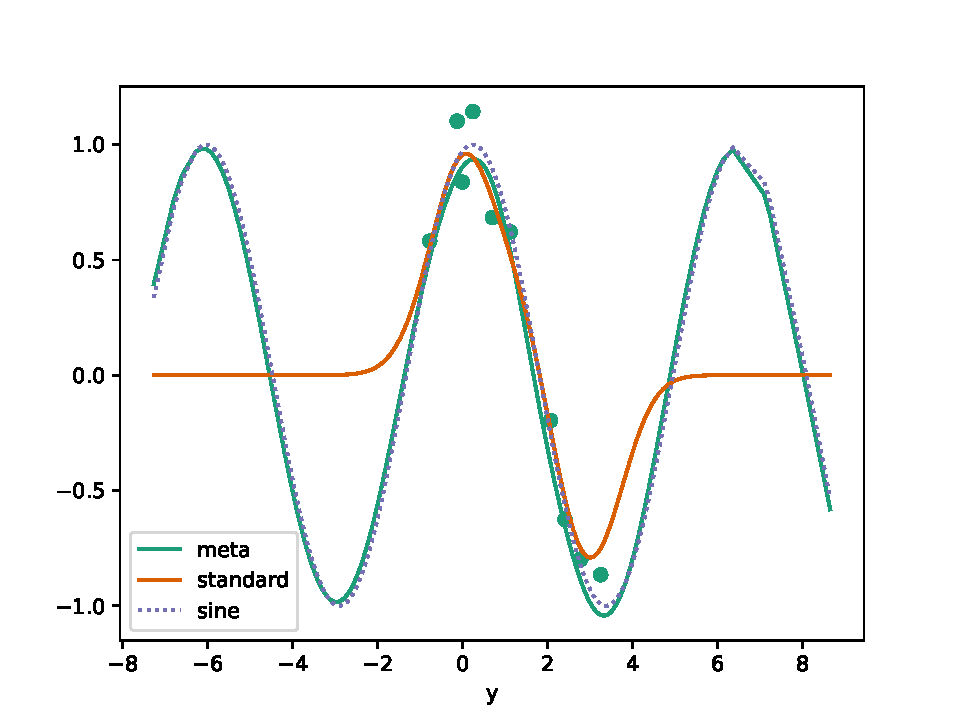
\includegraphics[width=\textwidth]{Figures/noise_1}
    \caption{Optimized hyper-parameters}
   \end{subfigure}
   \hfill
   \begin{subfigure}[b]{0.45\textwidth}
     \centering
     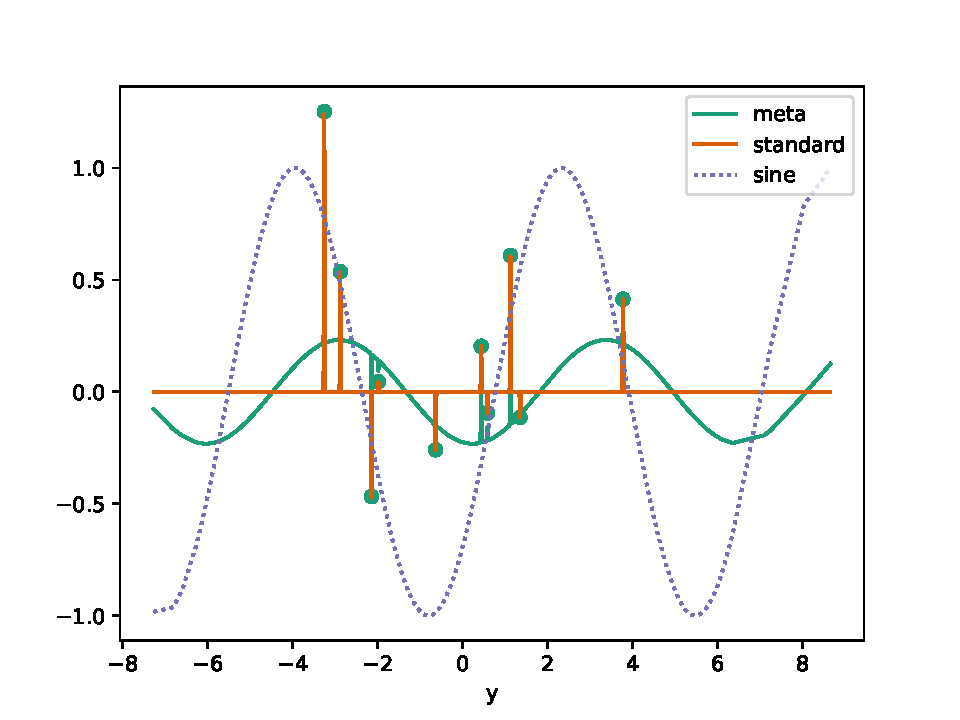
\includegraphics[width=\textwidth]{Figures/no_opt}
    \caption{No hyper-parameter tuning with small length scale and no regularization.}
   \end{subfigure}
    \caption{Demonstration}
\end{figure}

\section{Marco's Suggested Formulation}

\begin{itemize}
  \item Concatenated formulation gives the same result with my derivations, just machine precision differences.
\end{itemize}

The derivation is as follows,
\begin{equation}
  (\mathbf{A}\mathbf{w}-\mathbf{y})^\text{T}(\mathbf{A}\mathbf{w}-\mathbf{y}) + \lambda\mathbf{w}^\text{T}\mathbf{B}\mathbf{w},
\end{equation}

$\mathbf{A}:=[\mathbf{K}\boldsymbol{\psi}]\in \mR^{N\times(N+M)}$ and $B:=[\mathbf{K},0;0,0] \in \mR^{(N+M)\times(N+M)}$

Then the optimum parameters is found to be
\begin{equation}
  \hat{\mathbf{w}}=(\mathbf{A}^\text{T}\mathbf{A} + \lambda \mathbf{B}^\text{T})^{-1}\mathbf{A}^\text{T}\mathbf{y}.
\end{equation}


\section{Learning Curves and Additional Function Curve Effect}

\begin{figure}[h!]
   \centering
   \begin{subfigure}[b]{0.45\textwidth}
     \centering
     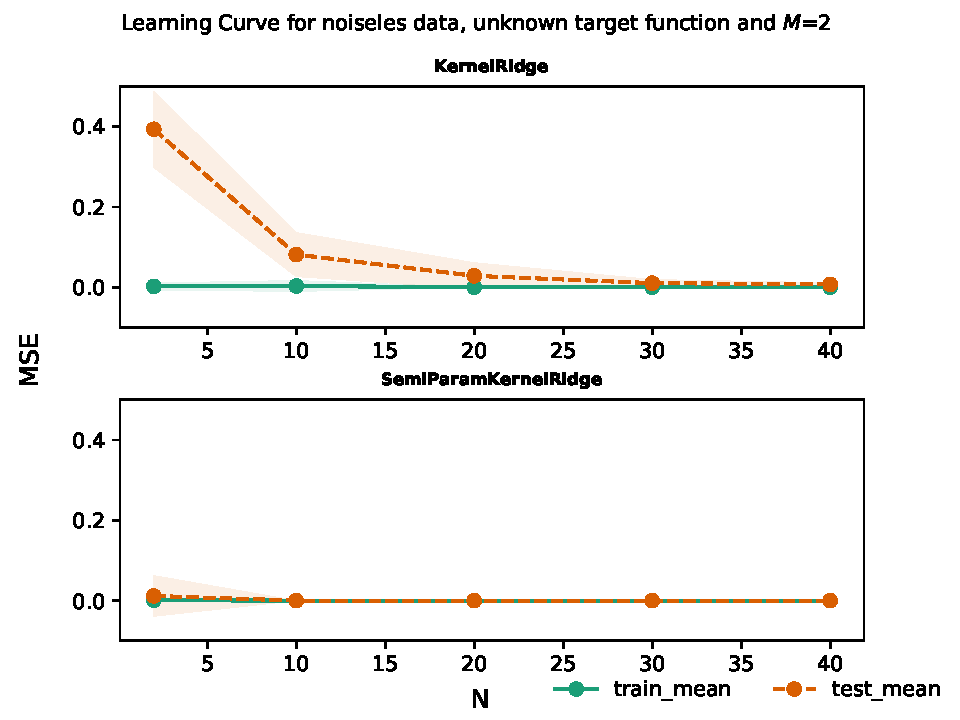
\includegraphics[width=\textwidth]{Figures/unknownnoiseless/learningcurve2}
     \caption{$M=2$}
   \end{subfigure}
   \hfill
   \begin{subfigure}[b]{0.45\textwidth}
     \centering
     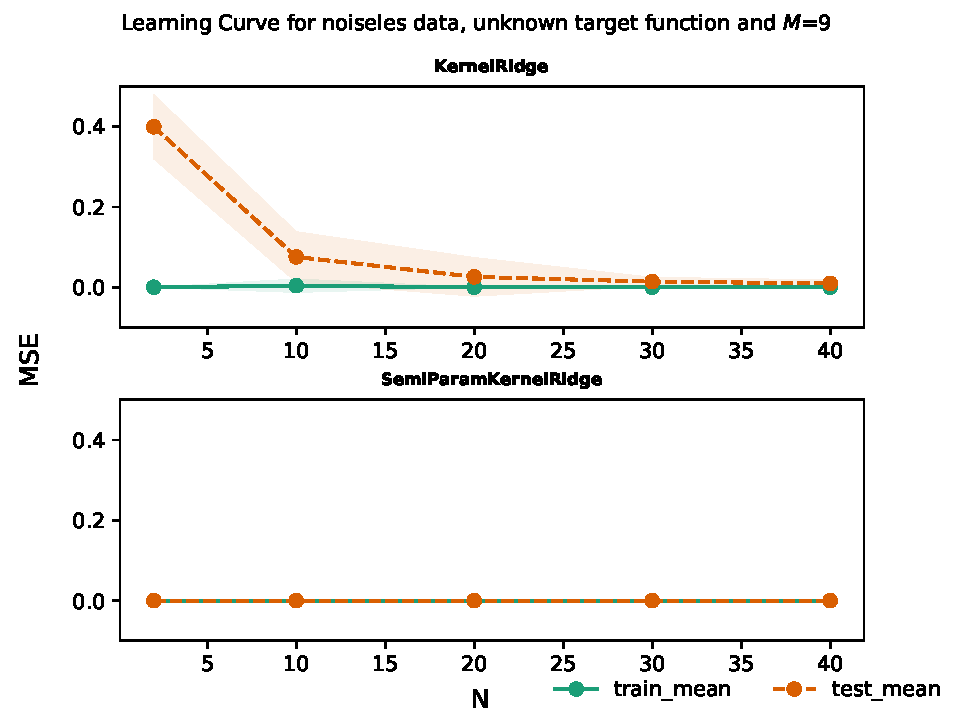
\includegraphics[width=\textwidth]{Figures/unknownnoiseless/learningcurve9}
     \caption{$M=9$}
   \end{subfigure}
   \caption{Noiseless Learning Curves for $M=2$ and $M=9$ Hyperparameters tuned and the drawn objective task is not present in $\boldsymbol{\psi}$.}
\end{figure}

\begin{figure}[h!]
   \centering
   \begin{subfigure}[b]{0.45\textwidth}
     \centering
     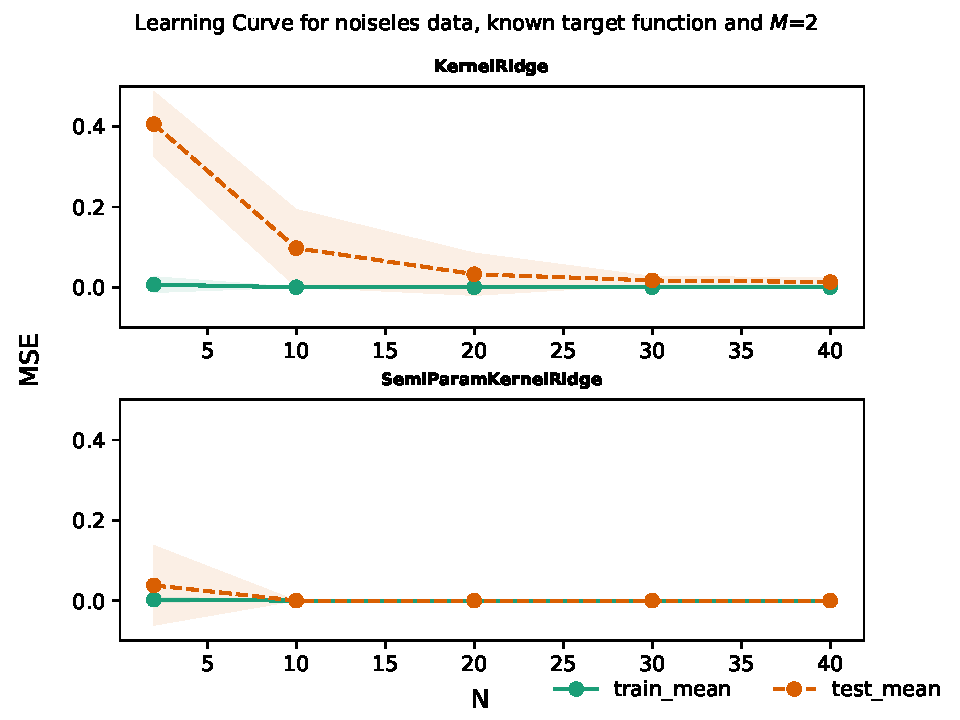
\includegraphics[width=\textwidth]{Figures/knownnoiseless/learningcurve2}
     \caption{$M=2$}
   \end{subfigure}
   \hfill
   \begin{subfigure}[b]{0.45\textwidth}
     \centering
     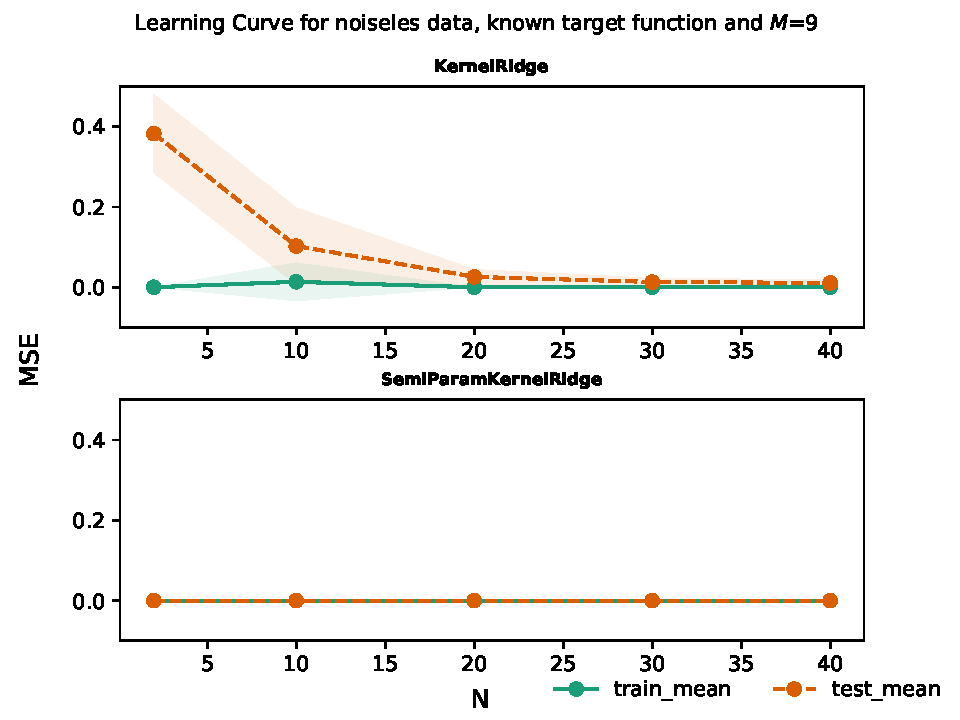
\includegraphics[width=\textwidth]{Figures/knownnoiseless/learningcurve9}
     \caption{$M=9$}
   \end{subfigure}
   \caption{Noiseless data Learning Curves for $M=2$ and $M=82$ Hyperparameters tuned and the drawn objective task is present in $\boldsymbol{\psi}$. }
\end{figure}

\begin{figure}[h!]
   \centering
   \begin{subfigure}[b]{0.45\textwidth}
     \centering
     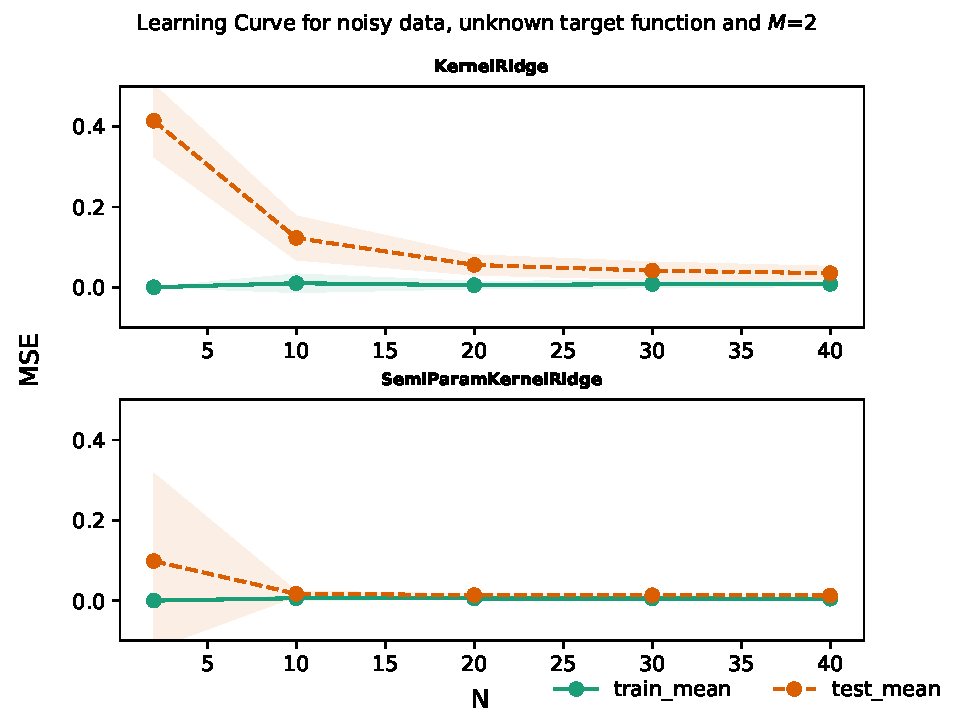
\includegraphics[width=\textwidth]{Figures/unknownnoisy/learningcurve2}
     \caption{$M=2$}
   \end{subfigure}
   \hfill
   \begin{subfigure}[b]{0.45\textwidth}
     \centering
     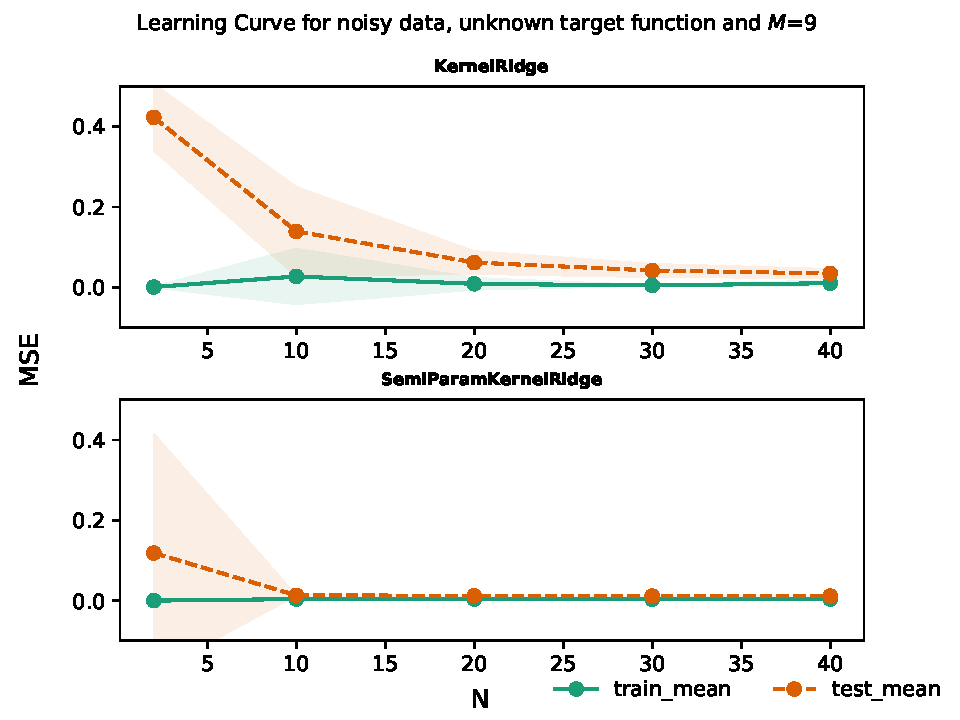
\includegraphics[width=\textwidth]{Figures/unknownnoisy/learningcurve9}
     \caption{$M=9$}
   \end{subfigure}
   \caption{Noisy data Learning Curves for $M=2$ and $M=9$ Hyperparameters tuned and the drawn objective task is not present in $\boldsymbol{\psi}$.}
\end{figure}

\begin{figure}[h!]
   \centering
   \begin{subfigure}[b]{0.45\textwidth}
     \centering
     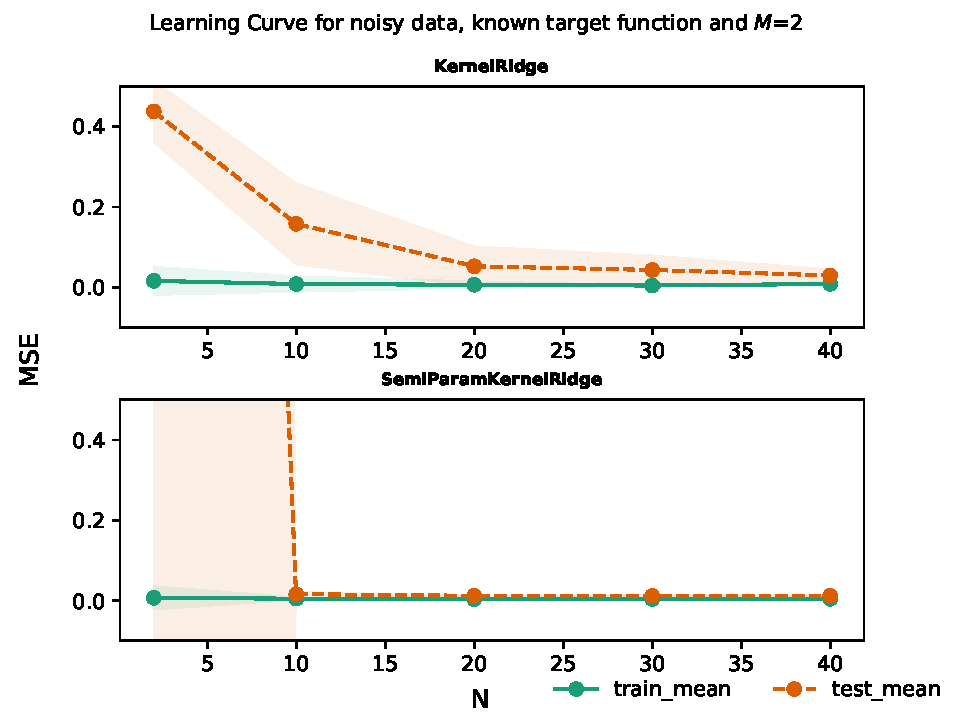
\includegraphics[width=\textwidth]{Figures/knownnoisy/learningcurve2}
     \caption{$M=2$}
   \end{subfigure}
   \hfill
   \begin{subfigure}[b]{0.45\textwidth}
     \centering
     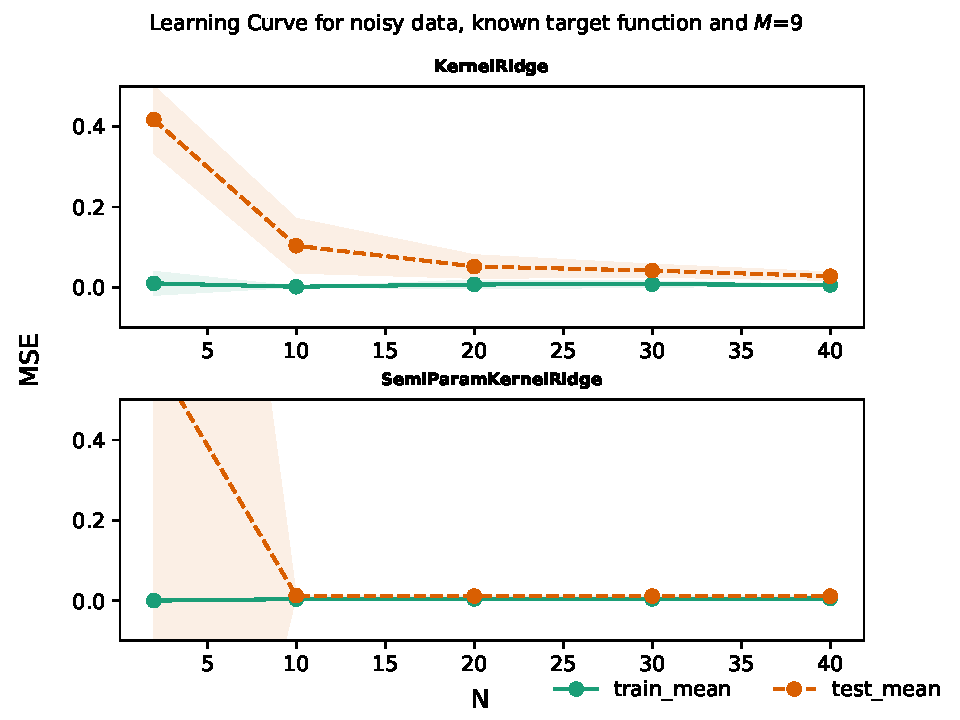
\includegraphics[width=\textwidth]{Figures/knownnoisy/learningcurve9}
     \caption{$M=9$}
   \end{subfigure}
   \caption{Noisy data Learning Curves for $M=2$ and $M=9$ Hyperparameters tuned and the drawn objective task is present in $\boldsymbol{\psi}$.}
\end{figure}

\begin{figure}[h!]
   \centering
   \begin{subfigure}[b]{0.45\textwidth}
     \centering
     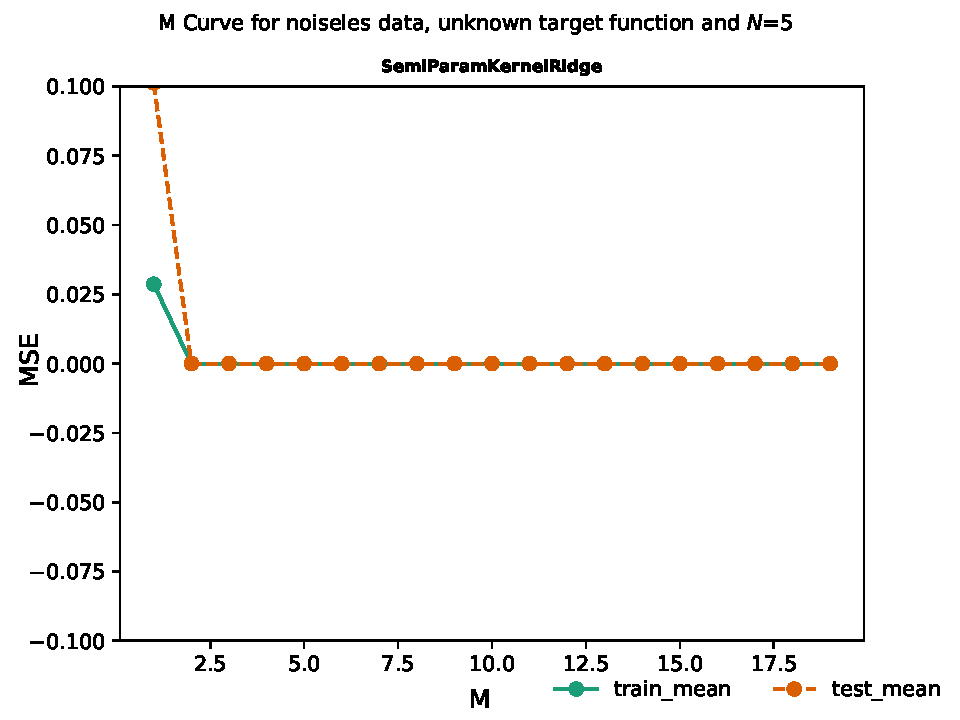
\includegraphics[width=\textwidth]{Figures/unknownnoiseless/Mcurve5}
     \caption{$N=5$}
   \end{subfigure}
   \hfill
   \begin{subfigure}[b]{0.45\textwidth}
     \centering
     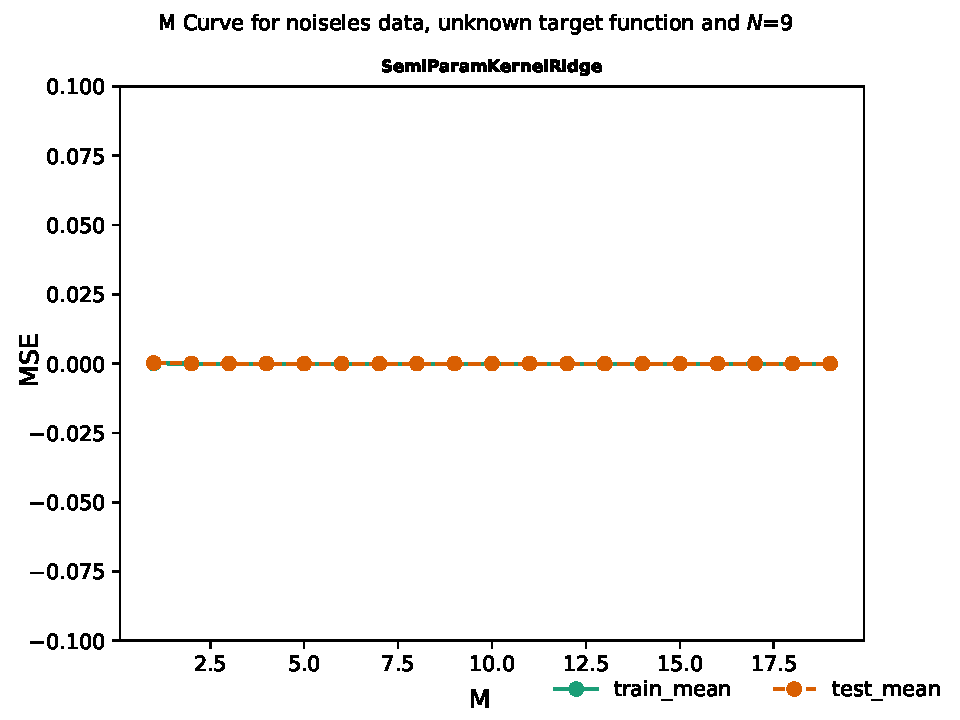
\includegraphics[width=\textwidth]{Figures/unknownnoiseless/Mcurve9}
     \caption{$N=9$}
   \end{subfigure}
   \caption{Noiseless data Complexity Curves for $N=5$ and $N=9$ Hyperparameters tuned and the drawn objective task is not present in $\boldsymbol{\psi}$.}
\end{figure}

\begin{figure}[h!]
   \centering
   \begin{subfigure}[b]{0.45\textwidth}
     \centering
     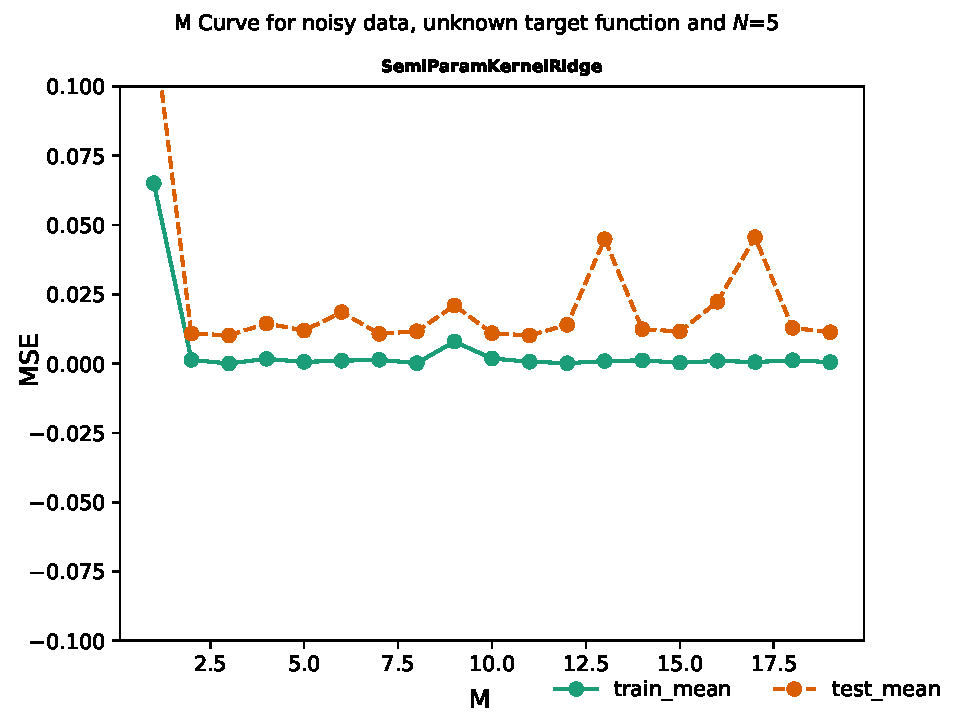
\includegraphics[width=\textwidth]{Figures/unknownnoisy/Mcurve5}
     \caption{$N=5$}
   \end{subfigure}
   \hfill
   \begin{subfigure}[b]{0.45\textwidth}
     \centering
     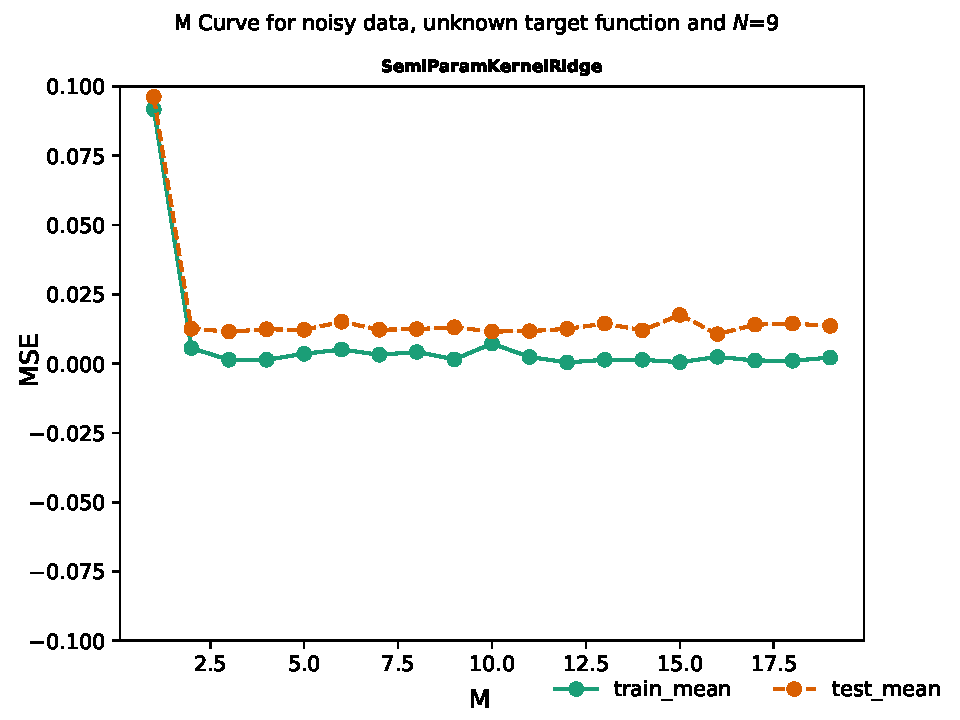
\includegraphics[width=\textwidth]{Figures/unknownnoisy/Mcurve9}
     \caption{$N=9$}
   \end{subfigure}
   \caption{Noisy data Complexity Curves for $N=5$ and $N=9$ Hyperparameters tuned and the drawn objective task is not present in $\boldsymbol{\psi}$.}
\end{figure}

\begin{figure}[h!]
   \centering
   \begin{subfigure}[b]{0.45\textwidth}
     \centering
     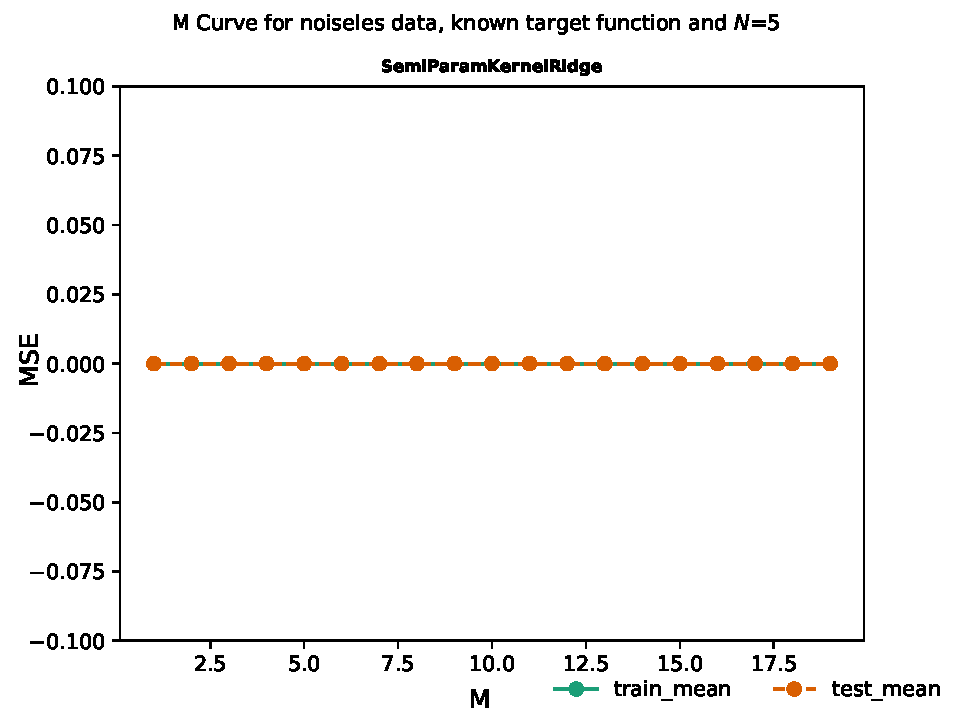
\includegraphics[width=\textwidth]{Figures/knownnoiseless/Mcurve5}
     \caption{$N=5$}
   \end{subfigure}
   \hfill
   \begin{subfigure}[b]{0.45\textwidth}
     \centering
     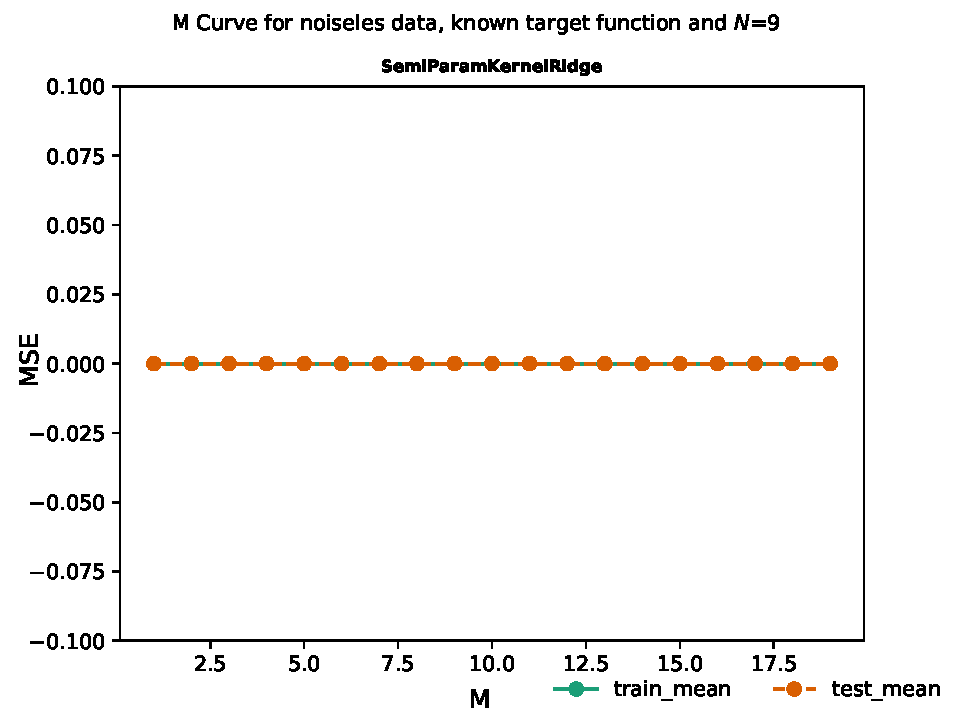
\includegraphics[width=\textwidth]{Figures/knownnoiseless/Mcurve9}
     \caption{$N=9$}
   \end{subfigure}
   \caption{Noiseless data Complexity Curves for $N=5$ and $N=9$ Hyperparameters tuned and the drawn objective task is present in $\boldsymbol{\psi}$.}
\end{figure}

\begin{figure}[h!]
   \centering
   \begin{subfigure}[b]{0.45\textwidth}
     \centering
     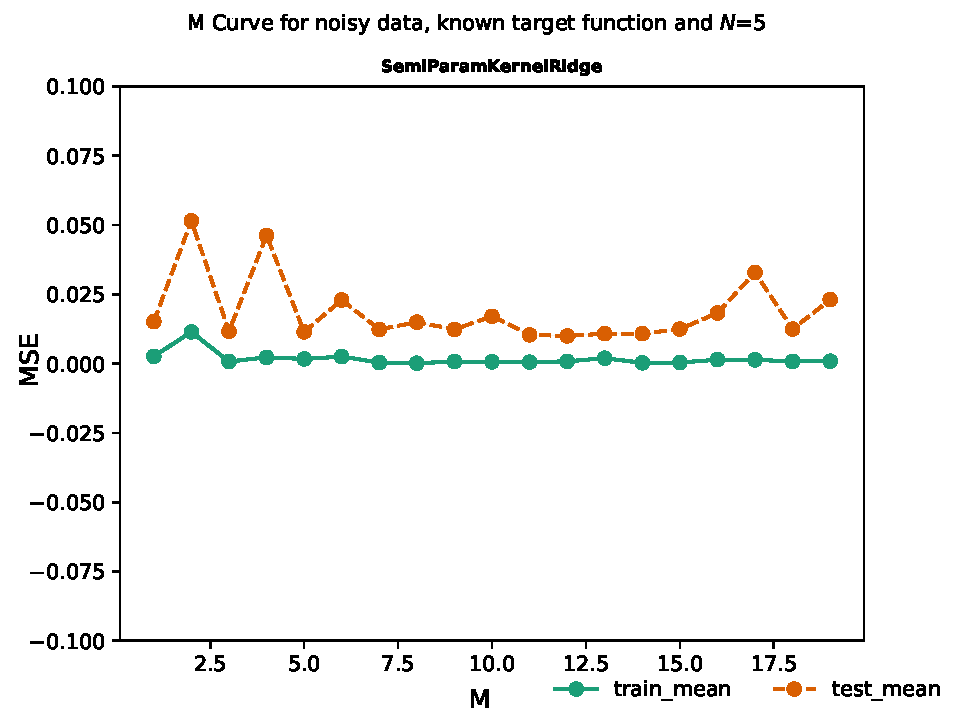
\includegraphics[width=\textwidth]{Figures/knownnoisy/Mcurve5}
     \caption{$N=5$}
   \end{subfigure}
   \hfill
   \begin{subfigure}[b]{0.45\textwidth}
     \centering
     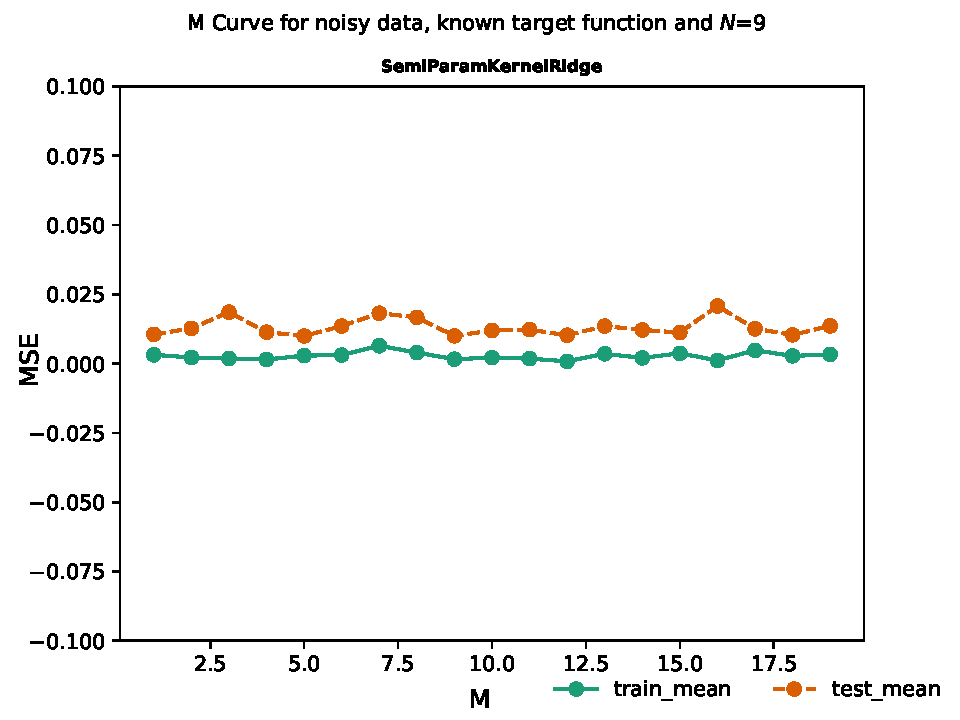
\includegraphics[width=\textwidth]{Figures/knownnoisy/Mcurve9}
     \caption{$N=9$}
   \end{subfigure}
   \caption{Noisy data Complexity Curves for $N=5$ and $N=9$ Hyperparameters tuned and the drawn objective task is present in $\boldsymbol{\psi}$.}
\end{figure}
\begin{itemize}
  \item Benefit of additional functions is evident.
  \item Looking at additional functions for unknown function case after having two functions we can almost go to zero test error. 
\end{itemize}

\section{Functional PCA}

Given the amount of functionals that can be present identifying  some form of representative form with less space but more information we can use dimensionality reduction techniques for functionals.

\begin{itemize}
  \item I am reading the Book Functional Data Analysis by Ramsay and Silverman.
  \item Smoothing and interpolation before using the data is essential.
  \item All the functionals have to be evaluated at the same input points $\{x_i\}_{i=1}^{N}$. In other words, we need to have the same grid. After putting them in to $\{f_i(\cdot)\}_{i=1}^P$
  \item For the functional PCA we want to find a set of K orthonormal functions so that the expension of each curve in terms of these basis functions approximates the curve as closely as possible.
  \item I do not see the point of writing the formulations I see in the book, but here is in a broad mathematical sense waht we are doing. Lets say our functions can be represented with linear combination of the values.
    \begin{equation}
      f_i = \{\sum_{j=1}^p \beta_j x_{ji}\}_{i=1}^N
    \end{equation}
  \item What functional PCA tries to do is to find the $\beta_j$ that maximizes the MSE with the constraint $||\beta_j||=1$ is satsified for every functional value.
  \item This way the largest variational modes are identified.
\end{itemize}

\begin{figure}[h!]
   \centering
   \begin{subfigure}[b]{0.45\textwidth}
     \centering
     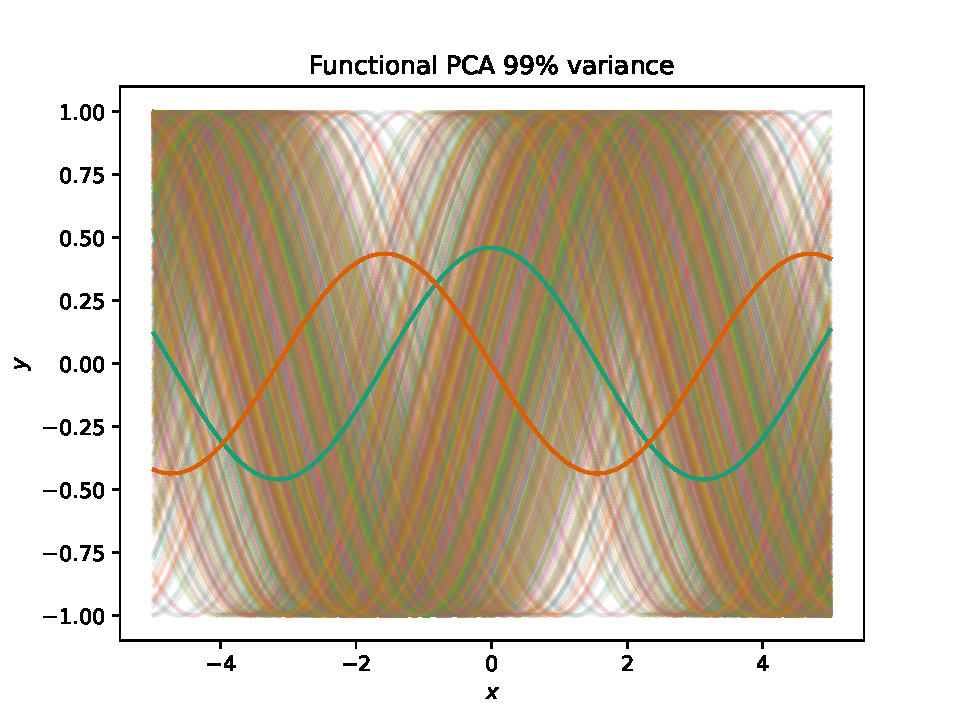
\includegraphics[width=\textwidth]{Figures/functional_pca_res/illustration}
     \caption{$P=2$}
   \end{subfigure}
   \hfill
   \begin{subfigure}[b]{0.45\textwidth}
     \centering
     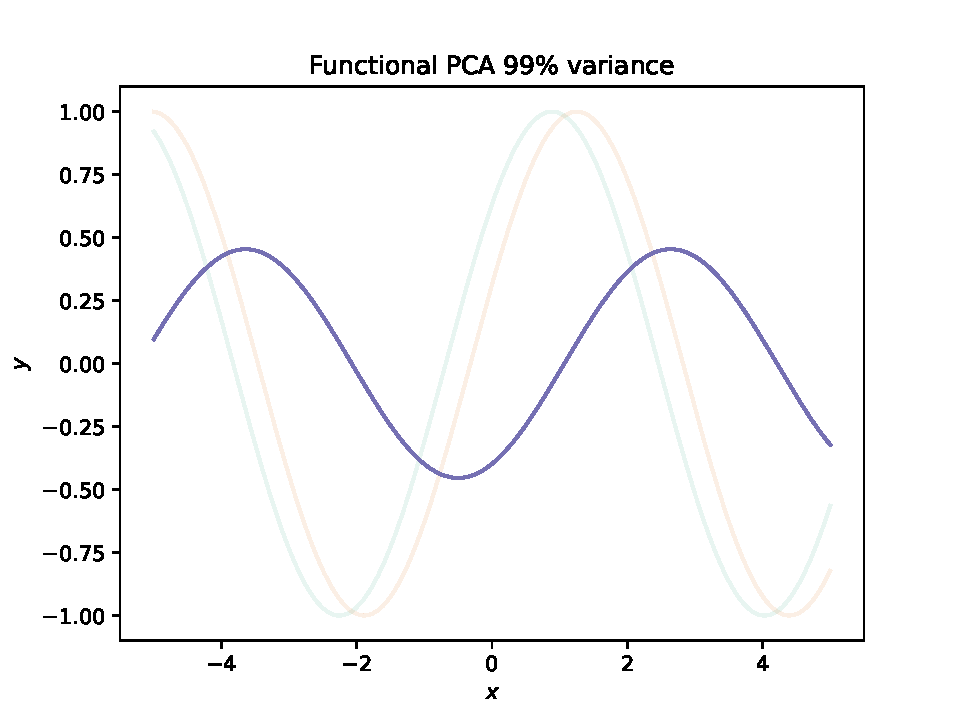
\includegraphics[width=\textwidth]{Figures/functional_pca_res/illustration-2}
     \caption{$P=9$}
   \end{subfigure}
   \caption{Observing the functional PCA results with 99\% of variance for different number of available functionals. Note that $P$ introduced here is analogous to $M$ in our above setting for SemiParametric method.}
\end{figure}

\begin{itemize}
  \item It is obvious that we can represent the whole range of sine to cosine with just two eigenfunctions. 
  \item What is more interesting is that we observed that for unknown task after $M=2$ we are able to obtain almost zero test error.
  \item After this observation I would like to use these PCA components as my $\psi_j(\cdot)$. But, know the same input point assumption is hindering flexibility.
\end{itemize}

\color{red}
\section{Learning Curves}

Some ideas on the similar method applied to learning curves.
\begin{itemize}
  \item Get learning curves for multiple hyper parameters for the same dataset then try to extrapolate one of them with the help of others.
  \item Try to extrapolate from untuned models to a tuned model.
\end{itemize}

\subsection{Ridge Regression Learning Curves}

From the Equation \ref{eq:data} observe data with $p(x)\sim\mathcal{N}(0,1)$ and $\epsilon\sim\mathcal{N}(0,1)$. Obtain the learning curves for different ridge parameters $\lambda$ for $N:{5,...,100}$

\begin{figure}[h!]
   \centering
   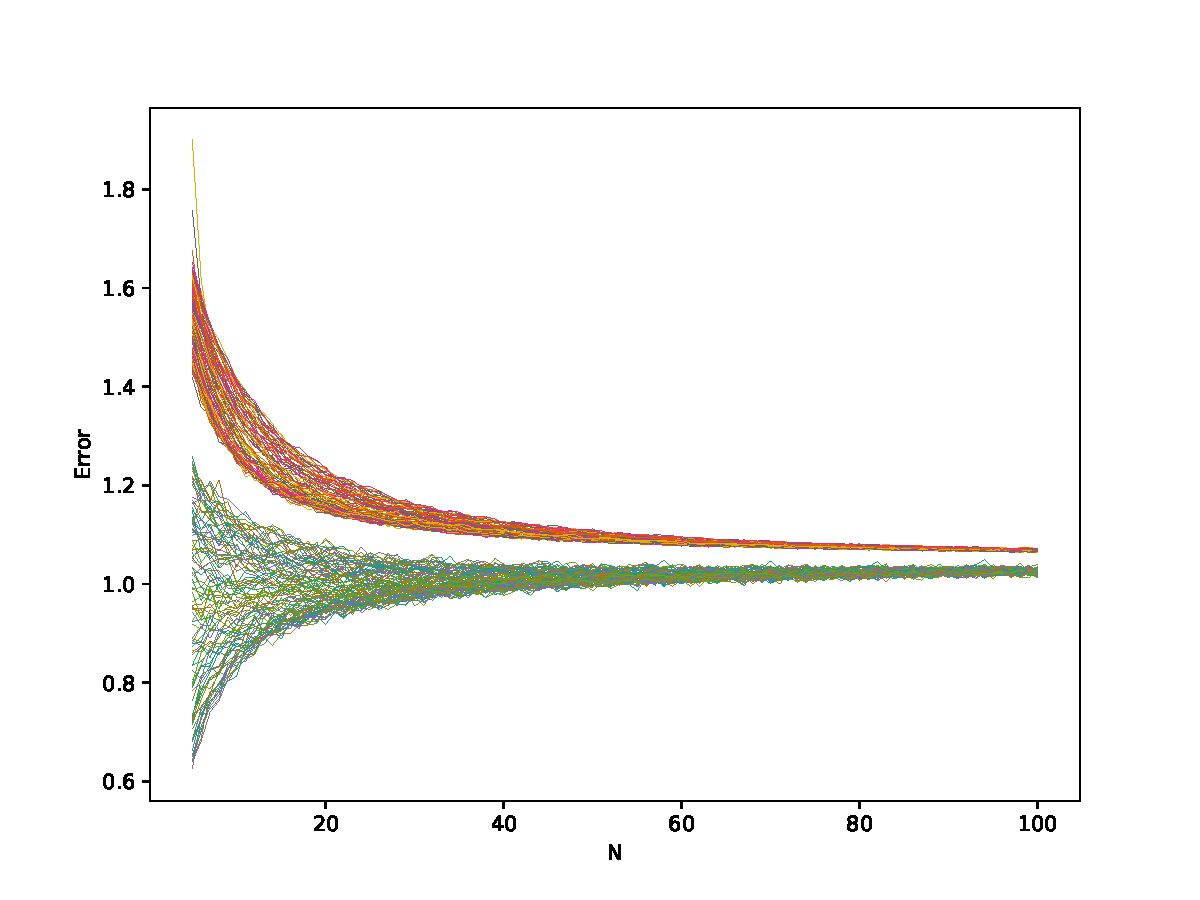
\includegraphics[width=\textwidth]{Figures/initial_study/lr_learning_curves.pdf}
   \caption{Learning Curves for Ridge Regression varying $\lambda$}
\end{figure}

\begin{figure}[h!]
   \centering
   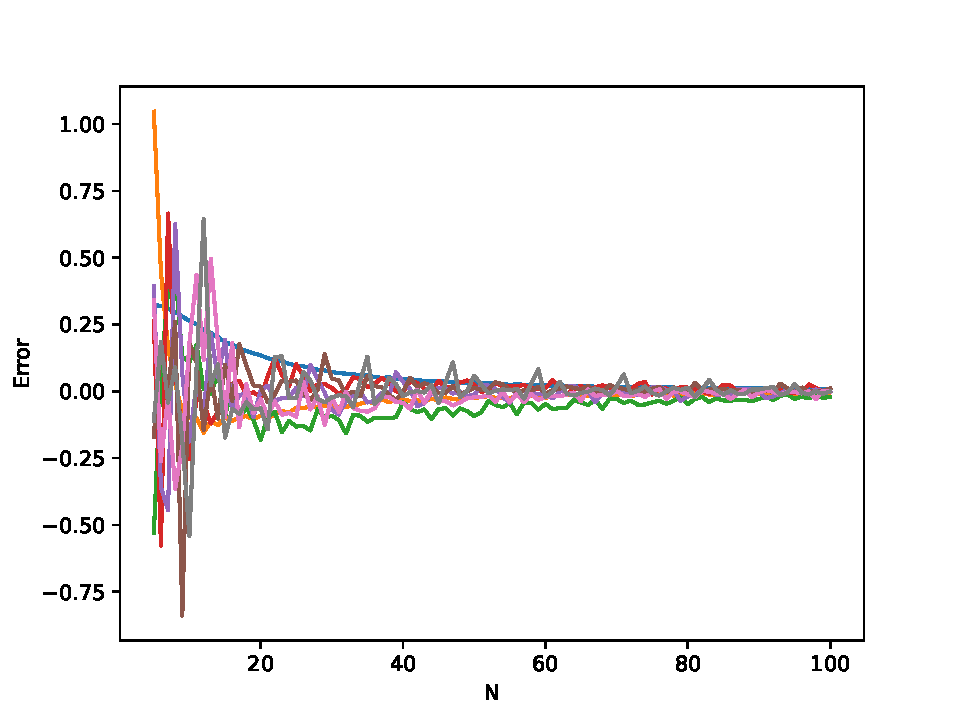
\includegraphics[width=\textwidth]{Figures/initial_study/lc_pca.pdf}
   \caption{PCA 99\% covering principle components (not smoothed!)$\lambda$}
\end{figure}

\begin{figure}[h!]
   \centering
   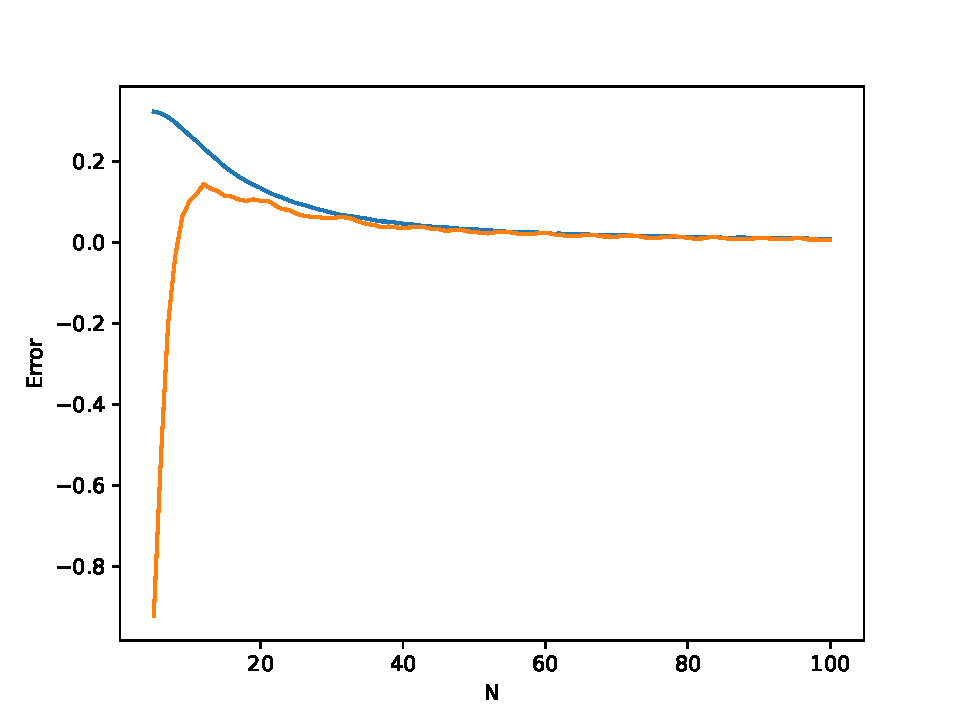
\includegraphics[width=\textwidth]{Figures/initial_study/smooth_pca.pdf}
   \caption{PCA 99\% covering principle components (smoothed!)$\lambda$}
\end{figure}

\begin{figure}[h!]
   \centering
   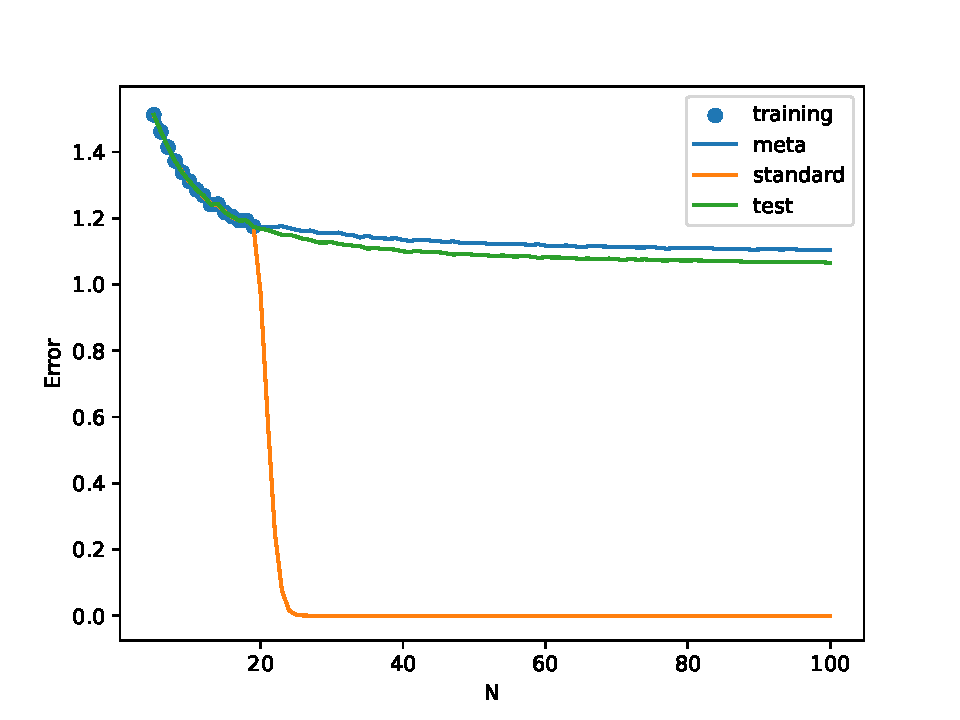
\includegraphics[width=\textwidth]{Figures/initial_study/lc_pred_funcs_1.pdf}
   \caption{Semi Parametric Kernel Ridge by using 1 other function. }
\end{figure}

\begin{figure}[h!]
   \centering
   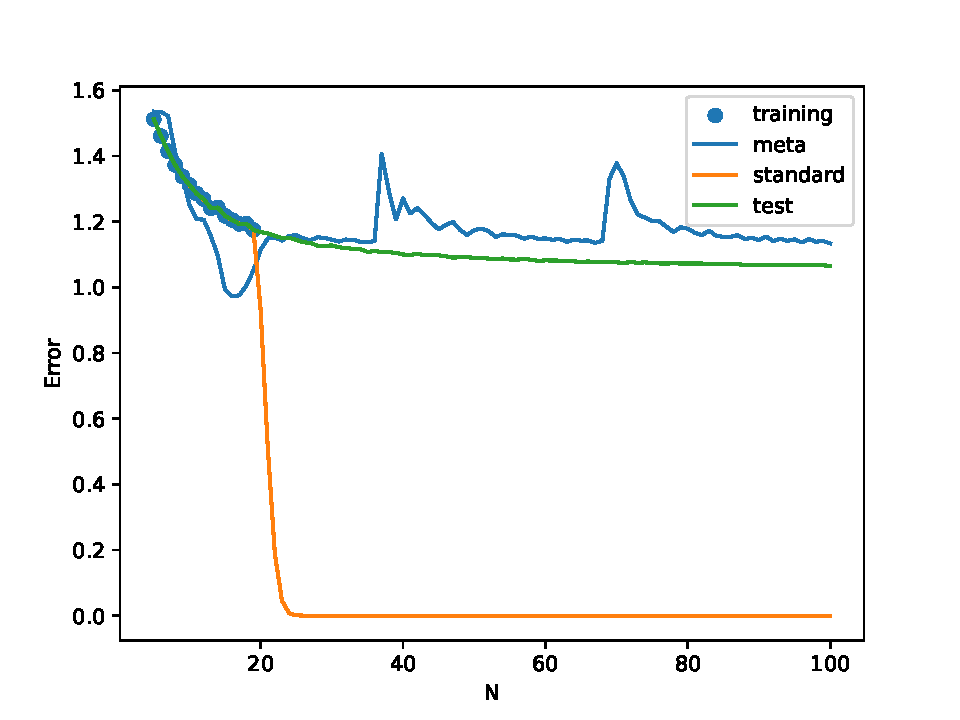
\includegraphics[width=\textwidth]{Figures/initial_study/lc_funcs_3.pdf}
   \caption{Semi Parametric Kernel Ridge by using 3 other functions. }
\end{figure}

\begin{figure}[h!]
   \centering
   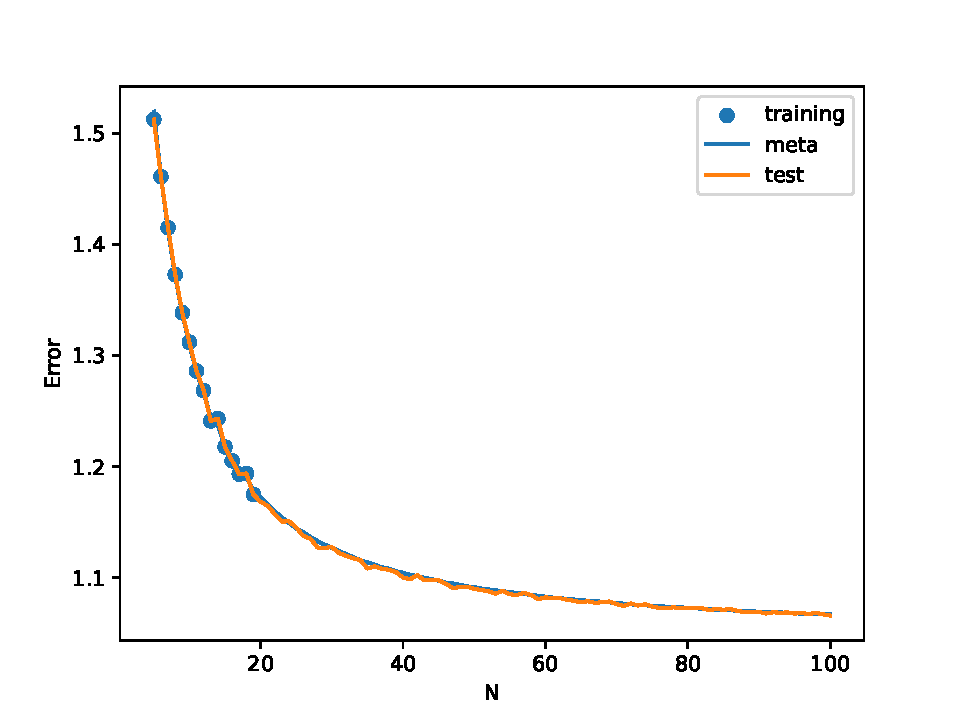
\includegraphics[width=\textwidth]{Figures/initial_study/lr_2_pca.pdf}
   \caption{Semi Parametric Kernel Ridge by using 2 PCA component. }
\end{figure}

\begin{figure}[h!]
   \centering
   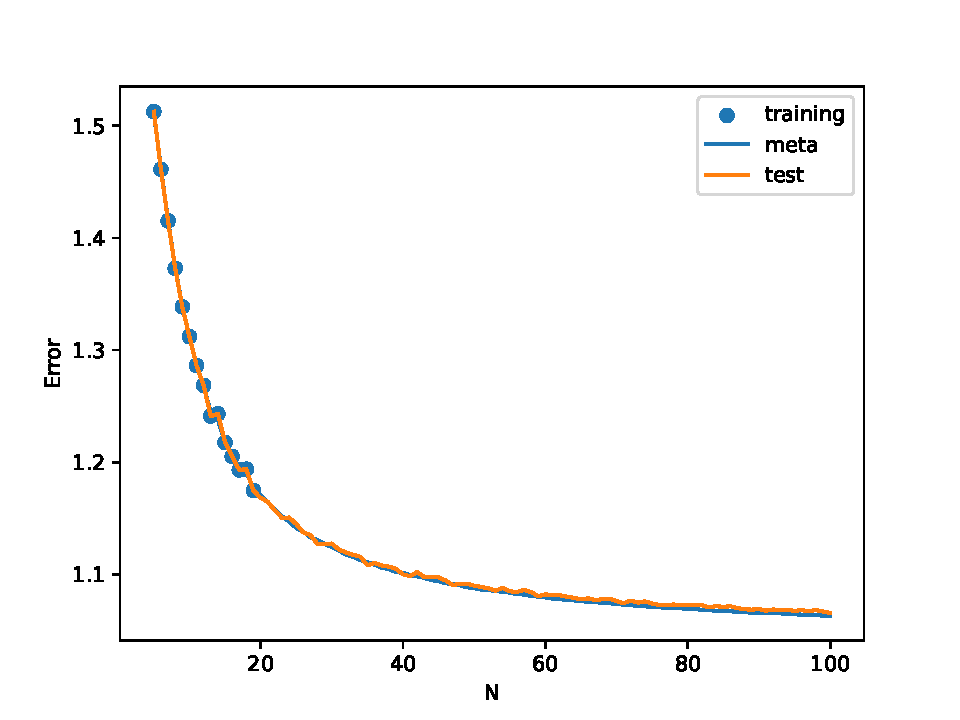
\includegraphics[width=\textwidth]{Figures/initial_study/lr_6_pca.pdf}
   \caption{Semi Parametric Kernel Ridge by using 6 PCA components. }
\end{figure}

NOTE: After the PCA mean of the functions are added to all the components.  The first principle component can deal relatively well with this thus the weight for it becomes just close to one! 

\begin{figure}[h!]
   \centering
   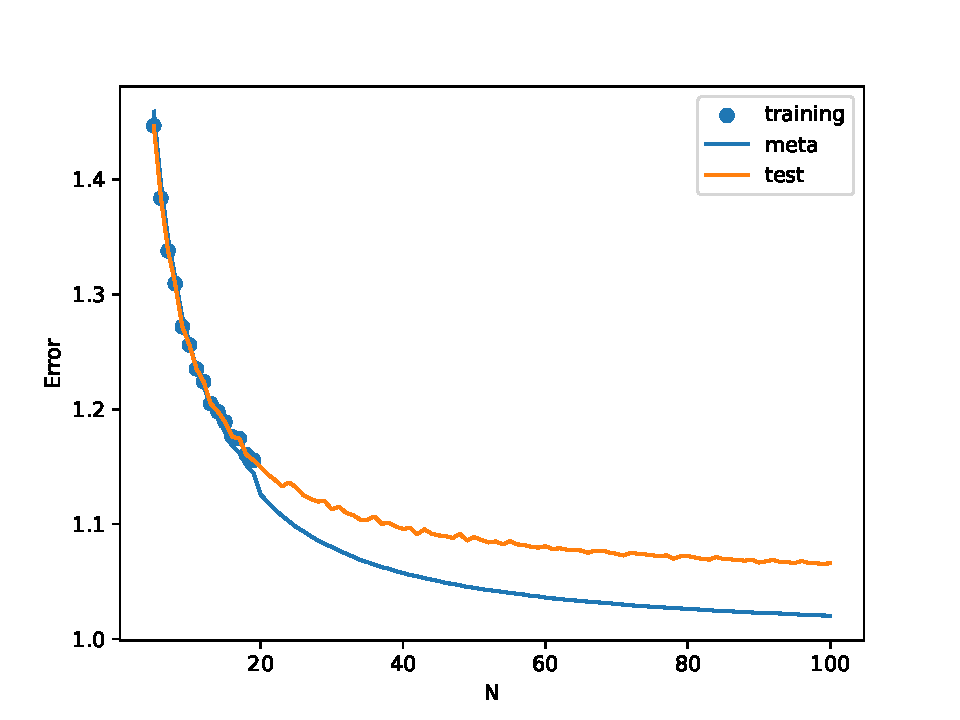
\includegraphics[width=\textwidth]{Figures/initial_study/lr_mean.pdf}
   \caption{Semi Parametric Kernel Ridge by using mean of the all components.}
\end{figure}


%\section{What does $\boldsymbol{\alpha}$ and $\boldsymbol{\beta}$}
%\begin{itemize}
%  \item $\boldsymbol{\alpha}$ by itself show the opposite behaviour that I would expect in Kernel Ridge. 
%  \item $\boldsymbol{\beta}$ is able to predict the objective easily.
%  \item Given that objective exists in $\boldsymbol{\psi}$ this method is able to find the internally best fit.
%  \item However, if the function is not representative of the underlying function the contribution of the additional information is not canceled.
%\end{itemize}
%
%\begin{figure}
%   \centering
%   \begin{subfigure}[b]{0.45\textwidth}
%     \centering
%     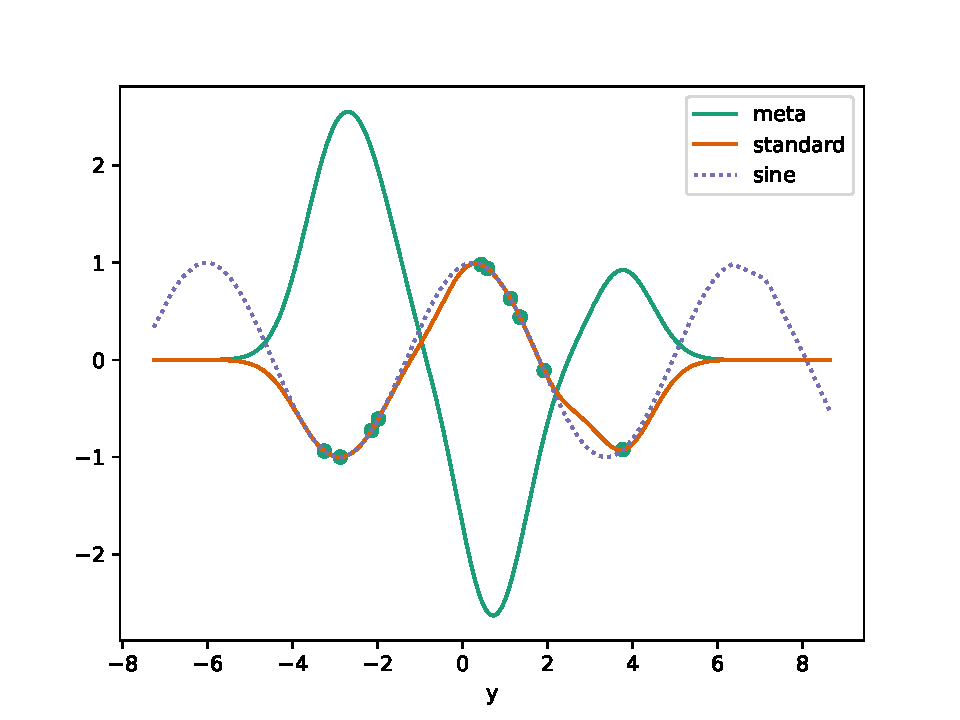
\includegraphics[width=\textwidth]{Figures/alpha}
%     \caption{Objective is present in $\boldsymbol{\psi}$}
%   \end{subfigure}
%   \hfill
%   \begin{subfigure}[b]{0.45\textwidth}
%     \centering
%     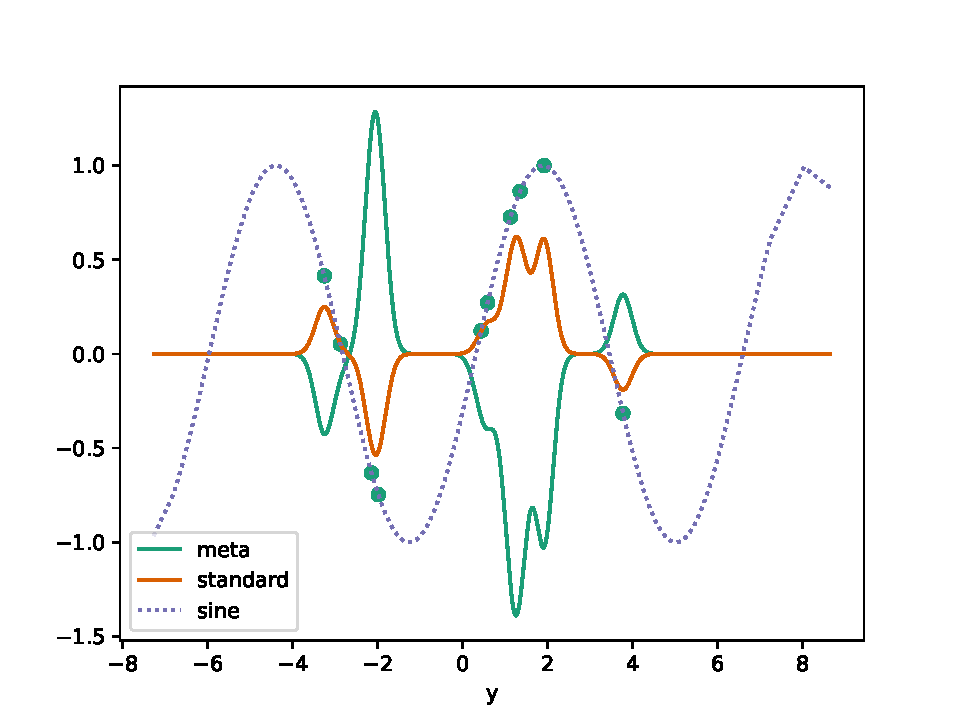
\includegraphics[width=\textwidth]{Figures/alpha_2}
%     \caption{Objective is not present in $\boldsymbol{\psi}$}
%   \end{subfigure}
%   \caption{$\boldsymbol{\alpha}$ Observations}
%\end{figure}
%
%\begin{figure}
%   \centering
%   \begin{subfigure}[b]{0.45\textwidth}
%     \centering
%     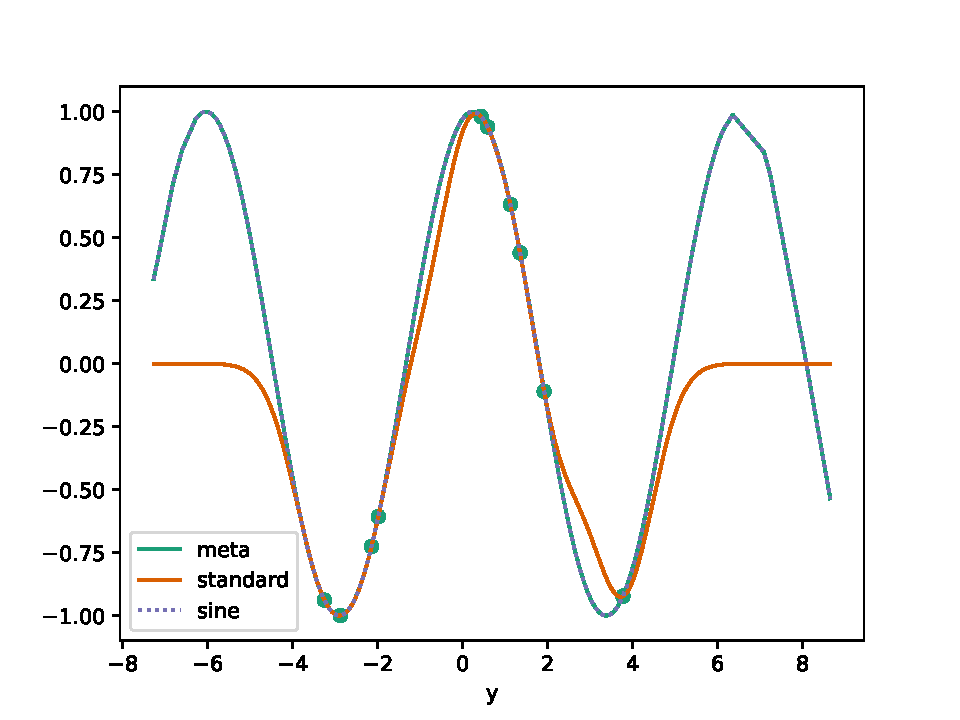
\includegraphics[width=\textwidth]{Figures/beta}
%     \caption{Objective is present in $\boldsymbol{\psi}$}
%   \end{subfigure}
%   \hfill
%   \begin{subfigure}[b]{0.45\textwidth}
%     \centering
%     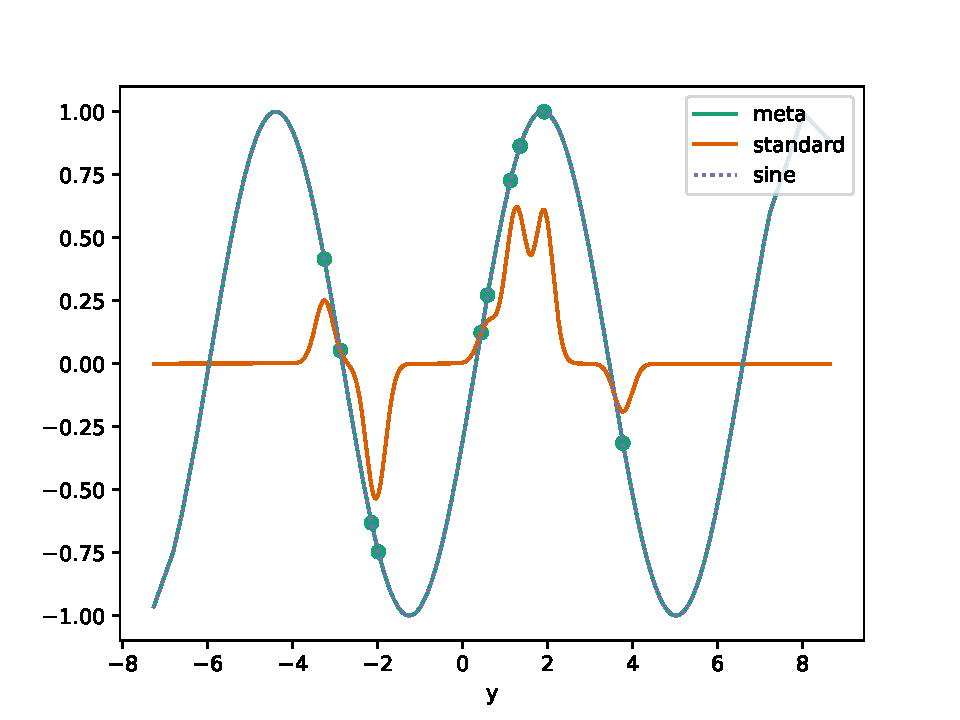
\includegraphics[width=\textwidth]{Figures/beta_2}
%     \caption{Objective is present in $\boldsymbol{\psi}$}
%   \end{subfigure}
%   \caption{$\boldsymbol{\beta}$ Observations}
%\end{figure}
%
%\begin{figure}
%  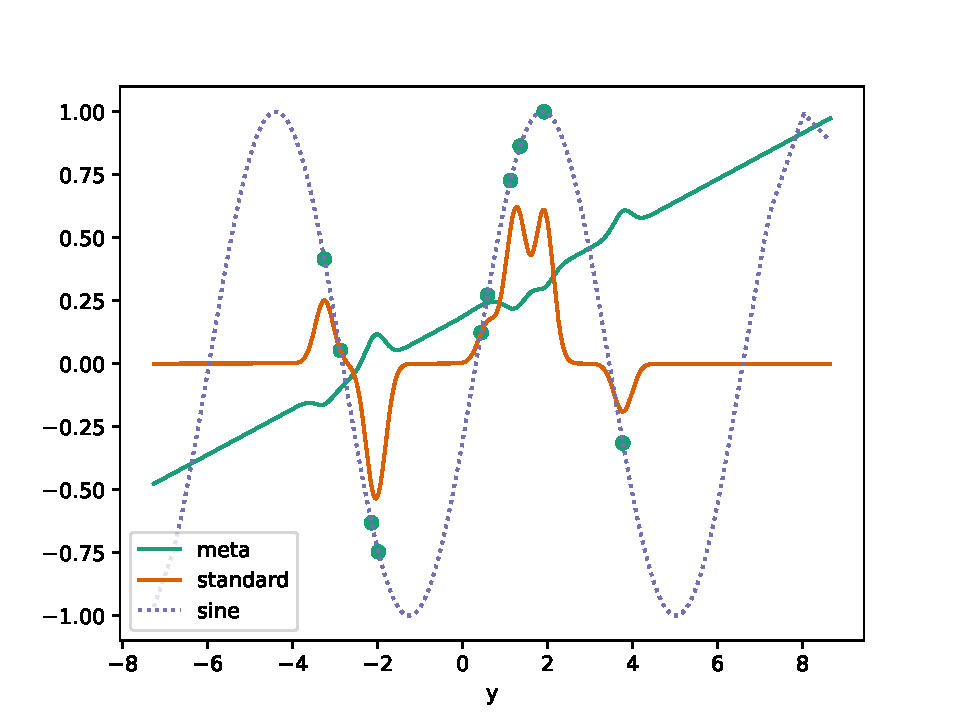
\includegraphics[width=0.5\textwidth]{Figures/linear_funcs}
%   \caption{Objective is present in $\boldsymbol{\psi}$}
%\end{figure}
%
%\section{Learning Curves for Varying $M$}
%
%\begin{itemize}
%  \item Hyper-parameters are tuned.
%  \item Some non-monotonic behaviour. I have no idea why that happens, need to put it to my own learning curve generator, to make sure not to have scikit learn bug.
%\end{itemize}
%
%\begin{figure}[!h]
%   \centering
%   \begin{subfigure}[b]{0.45\textwidth}
%     \centering
%     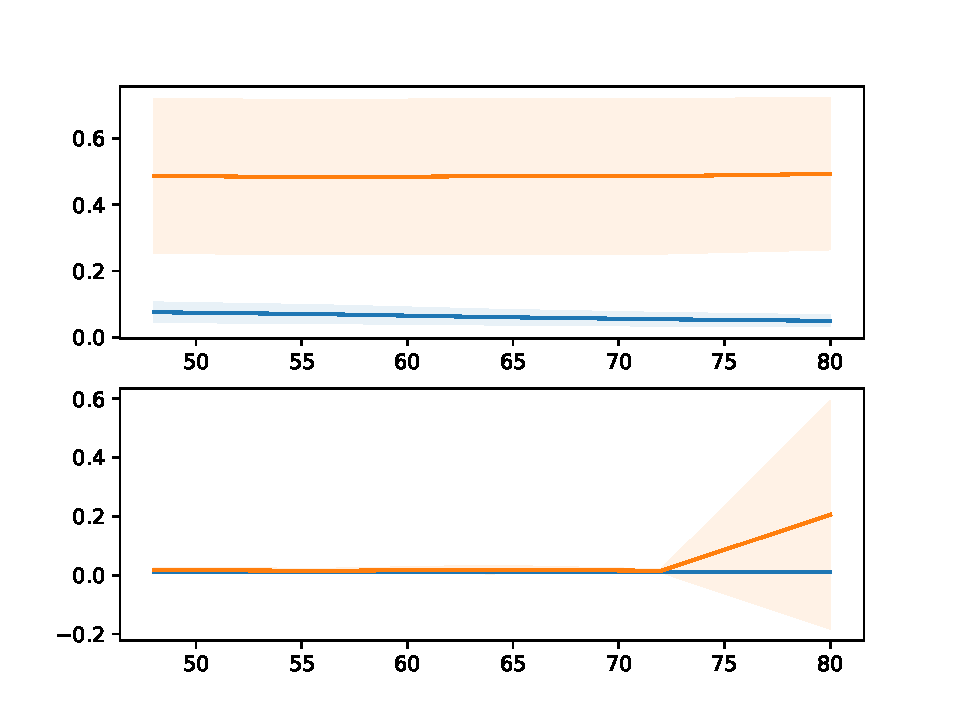
\includegraphics[width=\textwidth]{Figures/learning2}
%     \caption{2 functions for $\boldsymbol{\psi}$}
%   \end{subfigure}
%   \hfill
%   \begin{subfigure}[b]{0.45\textwidth}
%     \centering
%     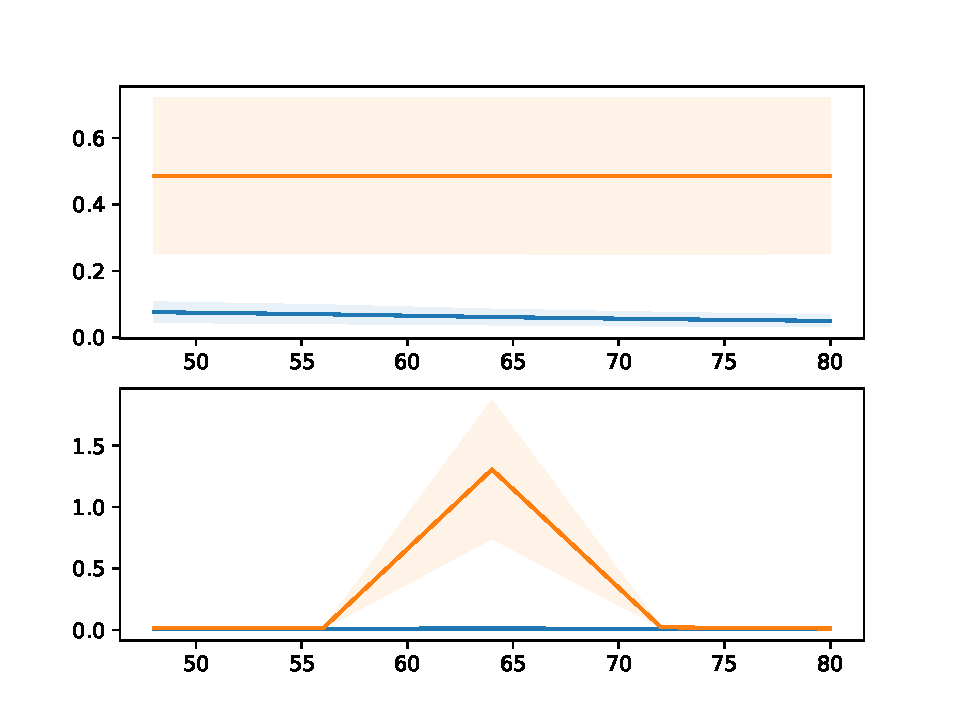
\includegraphics[width=\textwidth]{Figures/learning22}
%     \caption{22 functions for $\boldsymbol{\psi}$}
%   \end{subfigure}
%   \begin{subfigure}[b]{0.45\textwidth}
%     \centering
%     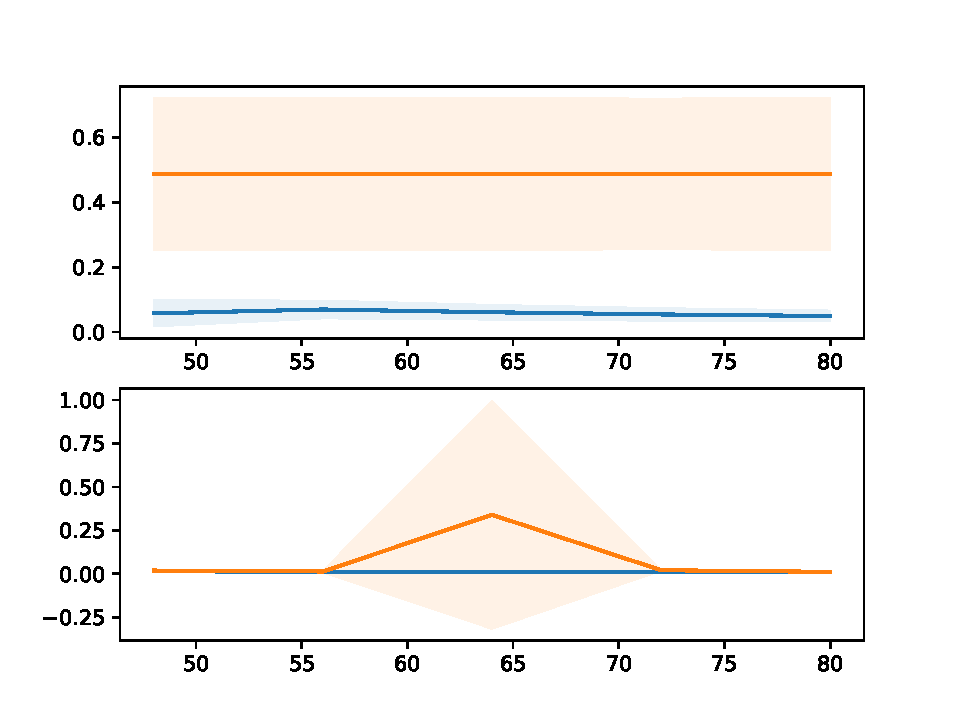
\includegraphics[width=\textwidth]{Figures/learning42}
%     \caption{42 functions for $\boldsymbol{\psi}$}
%   \end{subfigure}
%   \hfill
%   \begin{subfigure}[b]{0.45\textwidth}
%     \centering
%     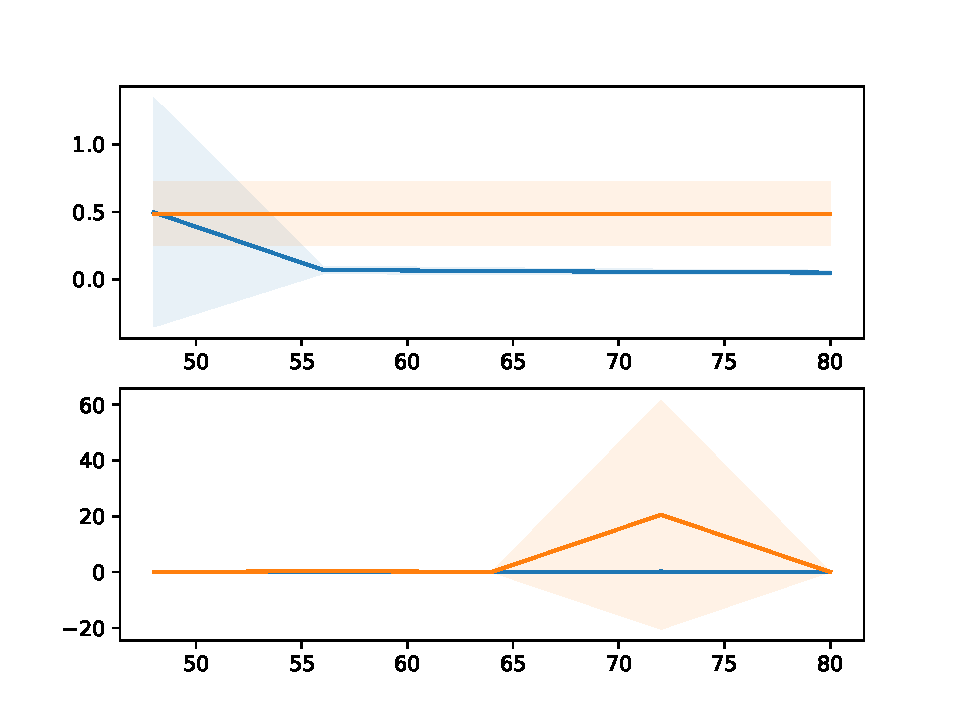
\includegraphics[width=\textwidth]{Figures/learning62}
%     \caption{62 functions for $\boldsymbol{\psi}$}
%   \end{subfigure}
%   \begin{subfigure}[b]{0.45\textwidth}
%     \centering
%     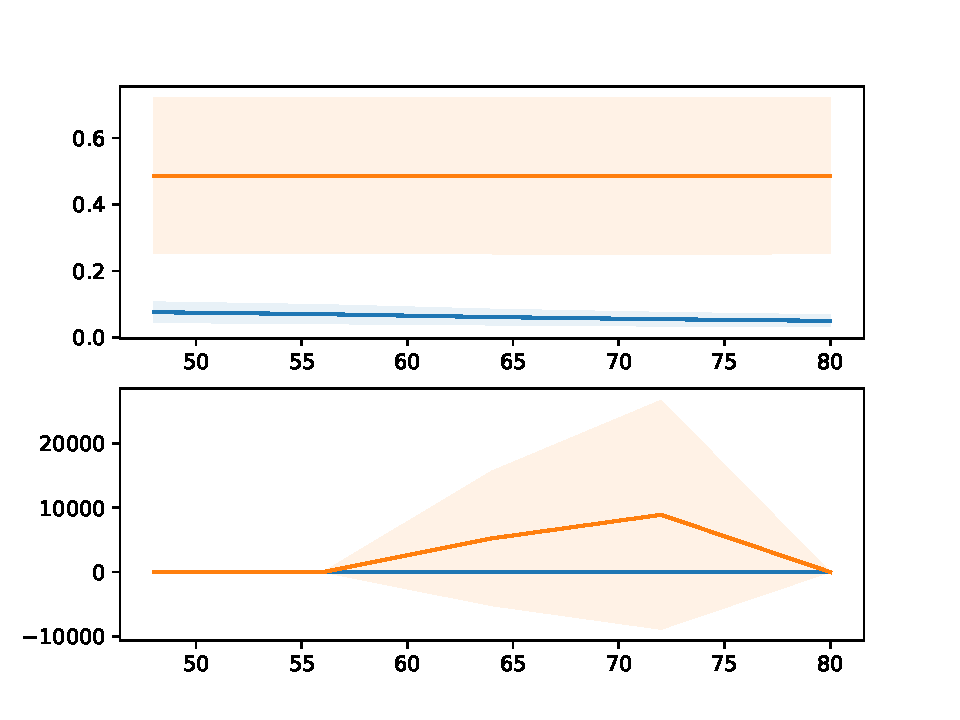
\includegraphics[width=\textwidth]{Figures/learning82}
%     \caption{82 functions for $\boldsymbol{\psi}$}
%   \end{subfigure}
%\end{figure}


\end{document}
